\documentclass[a4paper]{article}

\def\npart {III}
\def\nterm {Lent}
\def\nyear {2017}
\def\nlecturer {T. E. Forster}
\def\ncourse {Logic}

% Imports
\ifx \nextra \undefined
  \usepackage[pdftex,
    hidelinks,
    pdfauthor={Dexter Chua},
    pdfsubject={Cambridge Maths Notes: Part \npart\ - \ncourse},
    pdftitle={Part \npart\ - \ncourse},
  pdfkeywords={Cambridge Mathematics Maths Math \npart\ \nterm\ \nyear\ \ncourse}]{hyperref}
  \title{Part \npart\ - \ncourse}
\else
  \usepackage[pdftex,
    hidelinks,
    pdfauthor={Dexter Chua},
    pdfsubject={Cambridge Maths Notes: Part \npart\ - \ncourse\ (\nextra)},
    pdftitle={Part \npart\ - \ncourse\ (\nextra)},
  pdfkeywords={Cambridge Mathematics Maths Math \npart\ \nterm\ \nyear\ \ncourse\ \nextra}]{hyperref}

  \title{Part \npart\ - \ncourse \\ {\Large \nextra}}
\fi

\author{Lectured by \nlecturer \\\small Notes taken by Dexter Chua}
\date{\nterm\ \nyear}

\usepackage{alltt}
\usepackage{amsfonts}
\usepackage{amsmath}
\usepackage{amssymb}
\usepackage{amsthm}
\usepackage{booktabs}
\usepackage{caption}
\usepackage{enumitem}
\usepackage{fancyhdr}
\usepackage{graphicx}
\usepackage{mathtools}
\usepackage{microtype}
\usepackage{multirow}
\usepackage{pdflscape}
\usepackage{pgfplots}
\usepackage{siunitx}
\usepackage{tabularx}
\usepackage{tikz}
\usepackage{tkz-euclide}
\usepackage[normalem]{ulem}
\usepackage[all]{xy}

\pgfplotsset{compat=1.12}

\pagestyle{fancyplain}
\lhead{\emph{\nouppercase{\leftmark}}}
\ifx \nextra \undefined
  \rhead{
    \ifnum\thepage=1
    \else
      \npart\ \ncourse
    \fi}
\else
  \rhead{
    \ifnum\thepage=1
    \else
      \npart\ \ncourse\ (\nextra)
    \fi}
\fi
\usetikzlibrary{arrows}
\usetikzlibrary{decorations.markings}
\usetikzlibrary{decorations.pathmorphing}
\usetikzlibrary{positioning}
\usetikzlibrary{fadings}
\usetikzlibrary{intersections}
\usetikzlibrary{cd}

\newcommand*{\Cdot}{\raisebox{-0.25ex}{\scalebox{1.5}{$\cdot$}}}
\newcommand {\pd}[2][ ]{
  \ifx #1 { }
    \frac{\partial}{\partial #2}
  \else
    \frac{\partial^{#1}}{\partial #2^{#1}}
  \fi
}

% Theorems
\theoremstyle{definition}
\newtheorem*{aim}{Aim}
\newtheorem*{axiom}{Axiom}
\newtheorem*{claim}{Claim}
\newtheorem*{cor}{Corollary}
\newtheorem*{defi}{Definition}
\newtheorem*{eg}{Example}
\newtheorem*{fact}{Fact}
\newtheorem*{law}{Law}
\newtheorem*{lemma}{Lemma}
\newtheorem*{notation}{Notation}
\newtheorem*{prop}{Proposition}
\newtheorem*{thm}{Theorem}

\renewcommand{\labelitemi}{--}
\renewcommand{\labelitemii}{$\circ$}
\renewcommand{\labelenumi}{(\roman{*})}

\let\stdsection\section
\renewcommand\section{\newpage\stdsection}

% Strike through
\def\st{\bgroup \ULdepth=-.55ex \ULset}

% Maths symbols
\newcommand{\bra}{\langle}
\newcommand{\ket}{\rangle}

\newcommand{\N}{\mathbb{N}}
\newcommand{\Z}{\mathbb{Z}}
\newcommand{\Q}{\mathbb{Q}}
\renewcommand{\H}{\mathbb{H}}
\newcommand{\R}{\mathbb{R}}
\newcommand{\C}{\mathbb{C}}
\newcommand{\Prob}{\mathbb{P}}
\renewcommand{\P}{\mathbb{P}}
\newcommand{\E}{\mathbb{E}}
\newcommand{\F}{\mathbb{F}}
\newcommand{\cU}{\mathcal{U}}
\newcommand{\RP}{\mathbb{RP}}
\newcommand{\CP}{\mathbb{CP}}

\newcommand{\ph}{\,\cdot\,}

\DeclareMathOperator{\sech}{sech}
\DeclareMathOperator{\cosech}{cosech}
\DeclareMathOperator{\cosec}{cosec}

\DeclareMathOperator{\covol}{covol}
\DeclareMathOperator{\vol}{vol}

\let\Im\relax
\let\Re\relax
\DeclareMathOperator{\Im}{Im}
\DeclareMathOperator{\Re}{Re}
\DeclareMathOperator{\im}{im}
\DeclareMathOperator{\image}{image}
\DeclareMathOperator{\Ann}{Ann}

\DeclareMathOperator*{\res}{res}
\DeclareMathOperator{\Res}{Res}
\DeclareMathOperator{\Ind}{Ind}

\DeclareMathOperator{\tr}{tr}
\DeclareMathOperator{\diag}{diag}
\DeclareMathOperator{\rank}{rank}
\DeclareMathOperator{\card}{card}
\DeclareMathOperator{\spn}{span}
\DeclareMathOperator{\adj}{adj}

\DeclareMathOperator{\erf}{erf}
\DeclareMathOperator{\erfc}{erfc}

\DeclareMathOperator{\ord}{ord}
\DeclareMathOperator{\Sym}{Sym}

\DeclareMathOperator{\sgn}{sgn}
\DeclareMathOperator{\orb}{orb}
\DeclareMathOperator{\stab}{stab}
\DeclareMathOperator{\ccl}{ccl}

\DeclareMathOperator{\lcm}{lcm}
\DeclareMathOperator{\hcf}{hcf}

\DeclareMathOperator{\Int}{Int}
\DeclareMathOperator{\id}{id}

\DeclareMathOperator{\betaD}{beta}
\DeclareMathOperator{\gammaD}{gamma}
\DeclareMathOperator{\Poisson}{Poisson}
\DeclareMathOperator{\binomial}{binomial}
\DeclareMathOperator{\multinomial}{multinomial}
\DeclareMathOperator{\Bernoulli}{Bernoulli}
\DeclareMathOperator{\like}{like}

\DeclareMathOperator{\var}{var}
\DeclareMathOperator{\cov}{cov}
\DeclareMathOperator{\bias}{bias}
\DeclareMathOperator{\mse}{mse}
\DeclareMathOperator{\corr}{corr}

\DeclareMathOperator{\otp}{otp}
\DeclareMathOperator{\dom}{dom}

\DeclareMathOperator{\Root}{Root}
\DeclareMathOperator{\supp}{supp}
\DeclareMathOperator{\rel}{rel}
\DeclareMathOperator{\Hom}{Hom}
\DeclareMathOperator{\Aut}{Aut}
\DeclareMathOperator{\Gal}{Gal}
\DeclareMathOperator{\Mat}{Mat}
\DeclareMathOperator{\End}{End}
\DeclareMathOperator{\Char}{char}
\DeclareMathOperator{\ev}{ev}
\DeclareMathOperator{\St}{St}
\DeclareMathOperator{\Lk}{Lk}
\DeclareMathOperator{\disc}{disc}
\DeclareMathOperator{\Isom}{Isom}
\DeclareMathOperator{\length}{length}
\DeclareMathOperator{\energy}{energy}
\DeclareMathOperator{\area}{area}
\DeclareMathOperator{\Syl}{Syl}
\DeclareMathOperator{\cl}{cl}
\DeclareMathOperator{\fix}{fix}

\newcommand{\GL}{\mathrm{GL}}
\newcommand{\SL}{\mathrm{SL}}
\newcommand{\PGL}{\mathrm{PGL}}
\newcommand{\PSL}{\mathrm{PSL}}
\newcommand{\PSU}{\mathrm{PSU}}
\newcommand{\Or}{\mathrm{O}}
\newcommand{\SO}{\mathrm{SO}}
\newcommand{\U}{\mathrm{U}}
\newcommand{\SU}{\mathrm{SU}}

\renewcommand{\d}{\mathrm{d}}
\newcommand{\D}{\mathrm{D}}

\tikzset{->/.style = {decoration={markings,
                                  mark=at position 1 with {\arrow[scale=2]{latex'}}},
                      postaction={decorate}}}
\tikzset{<-/.style = {decoration={markings,
                                  mark=at position 0 with {\arrowreversed[scale=2]{latex'}}},
                      postaction={decorate}}}
\tikzset{<->/.style = {decoration={markings,
                                   mark=at position 0 with {\arrowreversed[scale=2]{latex'}},
                                   mark=at position 1 with {\arrow[scale=2]{latex'}}},
                       postaction={decorate}}}
\tikzset{->-/.style = {decoration={markings,
                                   mark=at position #1 with {\arrow[scale=2]{latex'}}},
                       postaction={decorate}}}
\tikzset{-<-/.style = {decoration={markings,
                                   mark=at position #1 with {\arrowreversed[scale=2]{latex'}}},
                       postaction={decorate}}}

\tikzset{circ/.style = {fill, circle, inner sep = 0, minimum size = 3}}
\tikzset{mstate/.style={circle, draw, blue, text=black, minimum width=0.7cm}}

\definecolor{mblue}{rgb}{0.2, 0.3, 0.8}
\definecolor{morange}{rgb}{1, 0.5, 0}
\definecolor{mgreen}{rgb}{0.1, 0.4, 0.2}
\definecolor{mred}{rgb}{0.5, 0, 0}

\def\drawcirculararc(#1,#2)(#3,#4)(#5,#6){%
    \pgfmathsetmacro\cA{(#1*#1+#2*#2-#3*#3-#4*#4)/2}%
    \pgfmathsetmacro\cB{(#1*#1+#2*#2-#5*#5-#6*#6)/2}%
    \pgfmathsetmacro\cy{(\cB*(#1-#3)-\cA*(#1-#5))/%
                        ((#2-#6)*(#1-#3)-(#2-#4)*(#1-#5))}%
    \pgfmathsetmacro\cx{(\cA-\cy*(#2-#4))/(#1-#3)}%
    \pgfmathsetmacro\cr{sqrt((#1-\cx)*(#1-\cx)+(#2-\cy)*(#2-\cy))}%
    \pgfmathsetmacro\cA{atan2(#2-\cy,#1-\cx)}%
    \pgfmathsetmacro\cB{atan2(#6-\cy,#5-\cx)}%
    \pgfmathparse{\cB<\cA}%
    \ifnum\pgfmathresult=1
        \pgfmathsetmacro\cB{\cB+360}%
    \fi
    \draw (#1,#2) arc (\cA:\cB:\cr);%
}
\newcommand\getCoord[3]{\newdimen{#1}\newdimen{#2}\pgfextractx{#1}{\pgfpointanchor{#3}{center}}\pgfextracty{#2}{\pgfpointanchor{#3}{center}}}

\def\Xint#1{\mathchoice
   {\XXint\displaystyle\textstyle{#1}}%
   {\XXint\textstyle\scriptstyle{#1}}%
   {\XXint\scriptstyle\scriptscriptstyle{#1}}%
   {\XXint\scriptscriptstyle\scriptscriptstyle{#1}}%
   \!\int}
\def\XXint#1#2#3{{\setbox0=\hbox{$#1{#2#3}{\int}$}
     \vcenter{\hbox{$#2#3$}}\kern-.5\wd0}}
\def\ddashint{\Xint=}
\def\dashint{\Xint-}


\usepackage{bussproofs}
\newcommand\intro[1]{\RightLabel{\scriptsize#1-int}}
\newcommand\intron[2]{\RightLabel{\scriptsize#1-int (#2)}}
\newcommand\elim[1]{\RightLabel{\scriptsize#1-elim}}

\newcommand\last{\mathsf{last}}
\newcommand\butlast{\mathsf{butlast}}
\newcommand\head{\mathsf{head}}
\newcommand\tail{\mathsf{tail}}
\newcommand\proj{\mathsf{proj}}
\newcommand\pair{\mathsf{pair}}
\newcommand\unpair{\mathsf{unpair}}
\newcommand\plus{\mathsf{plus}}
\newcommand\mult{\mathsf{mult}}
\newcommand\lexp{\mathsf{exp}}
\newcommand\K{\mathbb{K}}
\renewcommand\succ{\mathsf{succ}}
\newcommand\clet{\mathsf{let}\;}
\newcommand\cin{\;\mathsf{in}\;}
\newcommand\cid{\;\mathsf{id}\;}
\newcommand\cif{{\color{blue} \mathsf{if}\;}}
\newcommand\cthen{{\color{blue}\;\mathsf{then}\;}}
\newcommand\celse{{\color{blue}\;\mathsf{else}\;}}
\newcommand\con{\mathrm{con}}
\newcommand\ctrue{\mathsf{true}}
\newcommand\cons{\mathsf{cons}}
\newcommand\cfalse{\mathsf{false}}
\newcommand\ciszero{\mathsf{iszero}}
\newcommand\cfst{\mathsf{fst}}
\newcommand\csnd{\mathsf{snd}}
\newcommand\cnil{\mathsf{nil}}
\newcommand\cfact{\mathsf{fact}}
\newcommand\cmap{\mathsf{map}}
\newcommand\cnull{\mathsf{null}}
\newcommand\metafact{\mathsf{metafact}}
\newcommand\Yc{\mathsf{Y}}
\newcommand\cfind{\mathsf{find}}
\newenvironment{bprooftree}
  {\leavevmode\hbox\bgroup}
  {\DisplayProof\egroup}

\begin{document}
\maketitle
{\small
\setlength{\parindent}{0em}
\setlength{\parskip}{1em}
This course is the sequel to the Part II courses in Set Theory and Logic and in Automata and Formal Languages lectured in 2015-6. (It is already being referred to informally as ``Son of ST\&L and Automata \& Formal Languages''). Because of the advent of that second course this Part III course no longer covers elementary computability in the way that its predecessor (``Computability and Logic'') did, and this is reflected in the change in title. It will say less about Set Theory than one would expect from a course entitled `Logic'; this is because in Lent term Benedikt L\"owe will be lecturing a course entitled `Topics in Set Theory' and I do not wish to tread on his toes. Material likely to be covered include: advanced topics in first-order logic (Natural Deduction, Sequent Calculus, Cut-elimination, Interpolation, Skolemisation, Completeness and Undecidability of First-Order Logic, Curry-Howard, Possible world semantics, G\"odel's Negative Interpretation, Generalised quantifiers\ldots); Advanced Computability ($\lambda$-representability of computable functions, Tennenbaum's theorem, Friedberg-Muchnik, Baker-Gill-Solovay\ldots); Model theory background (ultraproducts, Los's theorem, elementary embeddings, omitting types, categoricity, saturation, Ehrenfeucht-Mostowski theorem\ldots); Logical combinatorics (Paris-Harrington, WQO and BQO theory at least as far as Kruskal's theorem on wellquasiorderings of trees\ldots). This is a new syllabus and may change in the coming months. It is entirely in order for students to contact the lecturer for updates.

\subsubsection*{Pre-requisites}
The obvious prerequisites from last year's Part II are Professor Johnstone's Set Theory and Logic and Dr Chiodo's Automata and Formal Languages, and I would like to assume that everybody coming to my lectures is on top of all the material lectured in those courses. This aspiration is less unreasonable than it may sound, since in 2016-7 both these courses are being lectured the term before this one, in Michaelmas; indeed supervisions for Part III students attending them can be arranged if needed: contact me or your director of studies. I am lecturing Part II Set Theory and Logic and I am even going to be issuing a ``Sheet 5'' for Set Theory and Logic, of material likely to be of interest to people who are thinking of pursuing this material at Part III. Attending these two Part II courses in Michaelmas is a course of action that may appeal particularly to students from outside Cambridge.
}
\tableofcontents

\section{Proof theory and constructive logic}
\subsection{Natural deduction}
The first person to have the notion of ``proof'' as a mathematical notion was probably G\"odel, and he needed this to write down the incompleteness theorem. The notion of proof he had was a very unintuitive notion. It is not very easy to manipulate, but they are easy to reason about.

In later years, people came up with more ``natural'' ways of defining proofs, and they are called natural deduction. In the formalism we learnt in IID Logic and Set Theory, we had three axioms only, and one rule of inference. In natural deduction, we have many rules of deduction.

We write or rules in the following form:
\[
  \begin{bprooftree}
    \AxiomC{$A$}
    \AxiomC{$B$}
    \intro{$\wedge$}
    \BinaryInfC{$A \wedge B$}
  \end{bprooftree}
\]
This says if we know $A$ and $B$ are true, then we can conclude $A \wedge B$. We call the things above the line the \term{premises}, and those below the line the \term{conclusions}. We can write out the other rules as follows:
\begin{center}
\begin{tabular}{cc}
   \begin{bprooftree}
    \AxiomC{$A$}
    \AxiomC{$B$}
    \intro{$\wedge$}
    \BinaryInfC{$A \wedge B$}
  \end{bprooftree} &
  \begin{bprooftree}
    \AxiomC{$A \wedge B$}
    \elim{$\wedge$}
    \UnaryInfC{$A$}
  \end{bprooftree}
  \begin{bprooftree}
    \AxiomC{$A \wedge B$}
    \elim{$\wedge$}
    \UnaryInfC{$B$}
  \end{bprooftree}\\[2em]
  \begin{bprooftree}
    \AxiomC{$A$}
    \intro{$\vee$}
    \UnaryInfC{$A \vee B$}
  \end{bprooftree}
  \begin{bprooftree}
    \AxiomC{$B$}
    \intro{$\vee$}
    \UnaryInfC{$A \vee B$}
  \end{bprooftree}\\[2em]
  &
  \begin{bprooftree}
    \AxiomC{$A$}
    \AxiomC{$A \to B$}
    \elim{$\to$}
    \BinaryInfC{$B$}
  \end{bprooftree}
\end{tabular}
\end{center}
Here we are separating these rules into two kinds --- the first column is the \term{introduction rules}. These tell us how we can \emph{introduce} a $\wedge$ or $\vee$ into our conclusions. The second column is the \term{elimination rules}. These tell us how we can \emph{eliminate} the $\wedge$ or $\to$ from our premises.

In general, we can think of these rules as ``LEGO pieces'', and we can use them to piece together to get ``LEGO assembles'', i.e.\ proofs.
\begin{eg}
  For example, we might have a proof that looks like
  \begin{prooftree}
    \AxiomC{$A$}
    \intro{$\vee$}
    \UnaryInfC{$A \vee B$}
    \AxiomC{$A \vee B \to C$}
    \elim{$\to$}
    \BinaryInfC{$C$}
  \end{prooftree}
  This corresponds to a proof that we can prove $C$ from $A$ and $A \vee B \to C$. Note that sometimes we are lazy and don't specify the rules we are using.
\end{eg}
Instead of trying to formally describe how we can put these rules together to form a proof, we will work through some examples as we go, and it should become clear.

We see that we are missing some rules from the table, as there are no introduction rule for $\to$ and elimination rule for $\vee$.

We work with $\to$ first. How we can prove $A \to B$? To do so, we assume $A$, and then try to prove $B$. If we can do so, then we have proved $A \to B$. But we cannot express this in the form of our previous rules. Instead what we want is some ``function'' that takes proof trees to proof trees.

The actual rule is as follows: suppose we have derivation that looks like
\begin{prooftree}
  \AxiomC{$A$}
  \noLine
  \UnaryInfC{$\rvdots$}
  \noLine
  \UnaryInfC{$C$}
\end{prooftree}
This is a proof of C under the assumption A. The $\to$-introduction rule says we can take this and turn it into a proof of $A \to C$.
\begin{prooftree}
  \AxiomC{$\rvdots$}
  \noLine
  \UnaryInfC{$A \to C$}
\end{prooftree}
This rule is not a LEGO piece. Instead, it is a magic wand that turns a LEGO piece into a LEGO piece.

But we do not want magic wands in our proofs. We want to figure out some more static way of writing this rule. We decided that it should look like this:
\begin{prooftree}
  \AxiomC{$[A]$}
  \noLine
  \UnaryInfC{$\rvdots$}
  \noLine
  \UnaryInfC{$C$}
  \intro{$\to$}
  \UnaryInfC{$A \to C$}
\end{prooftree}
Here the brackets denotes that we have given up on our assumption $A$ to obtain the conclusion $A \to C$. After doing so, we are no longer assuming $A$. When we work with complicated proofs, it is easy to get lost where we are eliminating the assumptions. So we would label them, and write this as, say
\begin{prooftree}
  \AxiomC{$[A]^1$}
  \noLine
  \UnaryInfC{$\rvdots$}
  \noLine
  \UnaryInfC{$C$}
  \intron{$\to$}{1}
  \UnaryInfC{$A \to C$}
\end{prooftree}

\begin{eg}
  We can transform our previous example to say
  \begin{prooftree}
    \AxiomC{$[A]^1$}
    \intro{$\vee$}
    \UnaryInfC{$A \vee B$}
    \AxiomC{$A \vee B \to C$}
    \elim{$\to$}
    \BinaryInfC{$C$}
    \intron{$\to$}{1}
    \UnaryInfC{$A \to C$}
  \end{prooftree}
  Originally, we had a proof that $A$ and $A \vee B \to C$ proves $C$. Now what we have is a proof that $A \vee B \to C$ implies $A \to C$.
\end{eg}

Next, we need an elimination rule of $A \vee B$. What should this be? Suppose we proved \emph{both} that $A$ proves $C$, \emph{and} $B$ proves $C$. Then if we know $A \vee B$, then we know $C$ must be true.

In other words, if we have
\begin{prooftree}
  \AxiomC{$A \vee B$}
  \AxiomC{$A$}
  \noLine
  \UnaryInfC{$\rvdots$}
  \noLine
  \UnaryInfC{$C$}
  \AxiomC{$B$}
  \noLine
  \UnaryInfC{$\rvdots$}
  \noLine
  \UnaryInfC{$C$}
  \TrinaryInfC{}
\end{prooftree}
then we can deduce $C$. We write this as
\begin{prooftree}
  \AxiomC{$A \vee B$}
  \AxiomC{$[A]$}
  \noLine
  \UnaryInfC{$\rvdots$}
  \noLine
  \UnaryInfC{$C$}
  \AxiomC{$[B]$}
  \noLine
  \UnaryInfC{$\rvdots$}
  \noLine
  \UnaryInfC{$C$}
  \elim{$\vee$}
  \TrinaryInfC{$C$}
\end{prooftree}
There is an obvious generalization to many disjunctions:
\begin{prooftree}
  \AxiomC{$A_1 \vee \cdots\vee A_n$}
  \AxiomC{$[A_1]$}
  \noLine
  \UnaryInfC{$\rvdots$}
  \noLine
  \UnaryInfC{$C$}
  \AxiomC{$[A_n]$}
  \noLine
  \UnaryInfC{$\rvdots$}
  \noLine
  \UnaryInfC{$C$}
  \elim{$\vee$}
  \TrinaryInfC{$C$}
\end{prooftree}
How about when we have an empty disjunction? The empty disjunction is just false. So this gives the rule
\begin{prooftree}
  \AxiomC{$\bot$}
  \UnaryInfC{$B$}
\end{prooftree}
In other words, we can prove anything assume falsehood. This is known as \term{ex falso sequitur quolibet}.

Note that we did not provide any rules for talking about negation. We do not need to do so, because we just take $\neg A$ to be $A \to \bot$.

So far, what we have described it \term{constructive propositional logic}. What is missing? We cannot use our system to prove the \term{law of excluded middle}, $A \vee \neg A$, or the \term{law of double negation} $\neg \neg A \to A$. It is not difficult to convince ourselves that it is impossible to prove these using the laws we have described above.

To obtain \term{classical propositional logic}, we need just one more rule, which is
\begin{prooftree}
  \AxiomC{$[A\to \bot]$}
  \noLine
  \UnaryInfC{$\rvdots$}
  \noLine
  \UnaryInfC{$\bot$}
  \UnaryInfC{$A$}
\end{prooftree}
If we add this, then we get classical propositional calculus, and it is a theorem that any truth-table-tautology (i.e.\ propositions that are always true for all possible values of $A, B, C$ etc) can be proved using natural deduction with the law of excluded middle.

\begin{eg}
  Suppose we want to prove
  \[
    A \to (B \to C) \to ((A \to B) \to (A \to C))
  \]
  How can we possibly prove this? The only way we can obtain this is to get something of the form
  \begin{prooftree}
    \AxiomC{$[A \to (B \to C)]$}
    \noLine
    \UnaryInfC{$\rvdots$}
    \noLine
    \UnaryInfC{$(A \to B) \to (A \to C)$}
    \intro{$\to$}
    \UnaryInfC{$A \to (B \to C) \to ((A \to B) \to (A \to C))$}
  \end{prooftree}
  Now the only way we can get the second-to-last conclusion is
  \begin{prooftree}
    \AxiomC{$A \to B$}
    \AxiomC{$[A]$}
    \noLine
    \BinaryInfC{$\rvdots$}
    \noLine
    \UnaryInfC{$C$}
    \UnaryInfC{$A \to C$}
  \end{prooftree}
  and then further eliminating $A \to B$ gives us $(A \to B) \to (A \to C)$. At this point we might see how we can patch them together to get a proof:
  \begin{prooftree}
    \AxiomC{$[A]^3$}
    \AxiomC{$[A \to (B \to C)]^1$}
    \BinaryInfC{$B \to C$}

    \AxiomC{$[A \to B]^2$}
    \AxiomC{$[A]^3$}
    \BinaryInfC{$B$}
    \BinaryInfC{$C$}
    \intron{$\to$}{3}
    \UnaryInfC{$A \to C$}
    \intron{$\to$}{2}
    \UnaryInfC{$(A \to B) \to (A \to C)$}
    \intron{$\to$}{1}
    \UnaryInfC{$A \to (B \to C) \to ((A \to B) \to (A \to C))$}
  \end{prooftree}
  Note that when we did $\to$-int (3), we consumed two copies of $A$ in one go. This is allowed, as an assumption doesn't become false after we use it once.

  However, some people study logical systems that do \emph{not} allow it, and demand that assumptions can only be used once. These are known as \term{resource logics}, one prominent example of which is \term{linear logic}.
\end{eg}

\begin{eg}
  Suppose we want to prove $A \to (B \to A)$. We have a proof tree
  \begin{prooftree}
    \AxiomC{$[A]^1$}
    \AxiomC{$[B]^2$}
    \BinaryInfC{$A$}
    \intron{$\to$}{2}
    \UnaryInfC{$B \to A$}
    \intron{$\to$}{1}
    \UnaryInfC{$A \to (B \to A)$}
  \end{prooftree}
  How did we manage to do the step from $A\;\; B$ to $A$? One can prove it as follows:
  \begin{prooftree}
    \AxiomC{$A$}
    \AxiomC{$B$}
    \intro{$\wedge$}
    \BinaryInfC{$A\wedge B$}
    \elim{$\wedge$}
    \UnaryInfC{$A$}
  \end{prooftree}
  but this is slightly unpleasant. It is redundant, and also breaks some nice properties of natural deduction we are going to prove later, e.g.\ the subformula property. So instead, we just put an additional \term{weakening rule} that just says we can drop any assumptions we like at any time.
\end{eg}

\begin{eg}
  Suppose we wanted to prove
  \[
    A \to (B \wedge C) \to ((A \to B) \wedge (A \to C)).
  \]
  This is indeed a truth-table tautology, as we can write out the truth table and see this is always true.

  If we try very hard, we will find out that we cannot prove it without using the law of excluded middle. In fact, this is not valid in constructive logic. Intuitively, the reason is that assuming $A$ is true, which of $B$ or $C$ is true can depend on why $A$ is true, and this it is impossible to directly prove that either $A \to B$ is true, or $A \to C$ is true.

  Of course, this is true in classical logic.
\end{eg}

\begin{ex}
  Prove the following:
  \begin{itemize}
    \item $(P \to Q) \to ((Q \to R) \to (P \to R))$
    \item $(A \to C) \to ((A \wedge B) \to C)$
    \item $((A \vee B) \to C) \to (A \to C)$
    \item $P \to (\neg P \to Q)$
    \item $A \to (A \to A)$
    \item $(P \vee Q) \to ((( P \to R) \wedge (Q \to S)) \to R \vee S)$
    \item $(P \wedge Q) \to ((( P \to R) \vee (Q \to S)) \to R \vee S)$
    \item $A \to ((((A \to B) \to B) \to C) \to C)$
    \item $((((P \to Q) \to P) \to P ) \to Q) \to Q$
  \end{itemize}
  The last two are hard.
\end{ex}

Instead of thinking of natural deduction as an actual logical theory, we often think of it as a ``platform'' that allows us to describe different logical theories, which we can do by introducing other connectives.

\begin{eg}
  For example, we might want to describe first-order logic. We can give introduction rules for $\exists$ as follows:
  \begin{prooftree}
    \AxiomC {$\varphi(t)$}
    \intro{$\exists$}
    \UnaryInfC{$\exists_x\varphi(x)$}
  \end{prooftree}
  Similarly, we can have an elimination rule for $\forall$ easily:
  \begin{prooftree}
    \AxiomC{$\forall_x \varphi(x)$}
    \elim{$\forall$}
    \UnaryInfC{$\varphi(t)$}
  \end{prooftree}
  The introduction rule for $\forall$ is a bit more complicated. The rule again looks something like
  \begin{prooftree}
    \AxiomC {$\varphi(x)$}
    \intro{$\forall$}
    \UnaryInfC{$\forall_x\varphi(x)$}
  \end{prooftree}
  but for such a proof to be valid, the $x$ must be ``arbitrary''. So we need an additional condition on this rule that there is no free occurrence of $x$'s.

  Finally, suppose we know $\exists_x \varphi(x)$. How can we use this to deduce some $p$? Suppose we know that $\varphi(x)$ implies $p$, and also $p$ does not depend on $x$. Then just knowing that there exists some $x$ such that $\varphi(x)$, we know $p$ must be true.
  \begin{prooftree}
    \AxiomC{$\exists_x \varphi(x)$}
    \AxiomC{$\varphi(x)$}
    \noLine
    \UnaryInfC{$\rvdots$}
    \noLine
    \UnaryInfC{$p$}
    \elim{$\exists$}
    \BinaryInfC{$p$}
  \end{prooftree}
  Again we need $x$ to be arbitrary in $p$. % maybe clarify this more
\end{eg}

\begin{eg}
  We can also use natural deduction for ``naive set theory'', which we will later find to be inconsistent. We can give an $\in$-introduction rule
  \begin{prooftree}
    \AxiomC{$\varphi(x)$}
    \intro{$\in$}
    \UnaryInfC{$x \in \{y : \varphi(y)\}$}
  \end{prooftree}
  and a similar elimination rule
  \begin{prooftree}
    \AxiomC{$x \in \{y: \varphi (y)\}$}
    \elim{$\in$}
    \UnaryInfC{$\varphi(x)$}
  \end{prooftree}
\end{eg}

One cannot expect that we can write down whatever introduction and elimination rule we like, and expect to get a sensible theory. For example, if we introduce a connective $\&$ with the following silly rules:
\begin{center}
  \begin{bprooftree}
    \AxiomC{$A$}
    \intro{$\&$}
    \UnaryInfC{$A \& B$}
  \end{bprooftree}
  \begin{bprooftree}
    \AxiomC{$A \& B$}
    \elim{$\&$}
    \UnaryInfC{$B$}
  \end{bprooftree}
\end{center}
then this would immediately give us a theory that proves anything we like.

There are in fact two problems with our introduction and elimination rules. The first is that once we use our $A$ to deduce $A \& B$, it is completely gone, and we cannot recover anything about $A$ from $A \& B$. The second problem is that, obviously, proving $A \& B$ doesn't really involve $B$ at all, but we can use $A \& B$ to deduce something about $B$.

In general, to obtain a sensible natural deduction theory, we need harmony.
\begin{defi}[Harmony]\index{harmony}
  We say a connective $\$ $ is \term{harmonious} if $\phi \$ \psi$ is the strongest assertion you can deduce from the assumptions in the rule of $\$ $-introduction, and $\phi \$ \psi$ is the weakest thing that implies the conclusion of the $\$ $-elimination rule.
\end{defi}
We will not make the notion more precise than this.

\begin{eg}
  The introduction and elimination rules for $\in$ we presented are certainly harmonious, because the conclusions and assumptions are in fact equivalent.

  One can also check that the introduction and elimination rules for $\wedge$ and $\vee$ are harmonious.
\end{eg}

\begin{eg}[Russel's paradox]
  In naive set theory, consider
  \[
    R = \{x: x \in x \to \bot\}.
  \]
  Then we can have the deductions
  \begin{prooftree}
    \AxiomC{$R \to R$}
    \AxiomC{$R \to R$}
    \elim{$\in$}
    \UnaryInfC{$R \in R \to \bot$}
    \elim{$\to$}
    \BinaryInfC{$\bot$}
  \end{prooftree}
  We can then move on to use this to deduce that $R \in R$:
  \begin{prooftree}
    \AxiomC{$[R \to R]^1$}
    \AxiomC{$[R \to R]^1$}
    \elim{$\in$}
    \UnaryInfC{$R \in R \to \bot$}
    \elim{$\to$}
    \BinaryInfC{$\bot$}
    \intron{$\to$}{1}
    \UnaryInfC{$R \in R \to \bot$}
    \intro{$\in$}
    \UnaryInfC{$R \in R$}
  \end{prooftree}
  Now we have proved $R \in R$. But we previously had a proof that $R \in R$ gives a contradiction. So what we are going to do is to make two copies of this proof:
  \begin{prooftree}
    \AxiomC{$[R \to R]^1$}
    \AxiomC{$[R \to R]^1$}
    \elim{$\in$}
    \UnaryInfC{$R \in R \to \bot$}
    \elim{$\to$}
    \BinaryInfC{$\bot$}
    \intron{$\to$}{1}
    \UnaryInfC{$R \in R \to \bot$}
    \intro{$\in$}
    \UnaryInfC{$R \in R$}
    \AxiomC{$[R \to R]^2$}
    \AxiomC{$[R \to R]^2$}
    \elim{$\in$}
    \UnaryInfC{$R \in R \to \bot$}
    \elim{$\to$}
    \BinaryInfC{$\bot$}
    \intron{$\to$}{2}
    \UnaryInfC{$R \in R \to \bot$}
    \elim{$\to$}
    \BinaryInfC{$\bot$}
  \end{prooftree}
  So we showed that we have an inconsistent theory.

  Note that we didn't use a lot of ``logical power'' here. We didn't use the law of excluded middle, so this contradiction manifests itself even in the case of constructive logic. Moreover, we didn't really use many axioms of naive set theory. We didn't even need things like extensionality for this to work.
\end{eg}

Now we notice that this proof is rather weird. We first had an $\to$-introduction (2), and then subsequently eliminated it immediately. In general, if we have a derivation of the form
\begin{prooftree}
  \AxiomC{$P$}
  \noLine
  \UnaryInfC{$\rvdots$}
  \noLine
  \UnaryInfC{$Q$}
  \intro{$\to$}
  \UnaryInfC{$P \to Q$}
  \AxiomC{$\rvdots$}
  \noLine
  \UnaryInfC{$P$}
  \elim{$\to$}
  \BinaryInfC{$Q$}
\end{prooftree}
We can just move the second column to the top of the first to get
\begin{prooftree}
  \AxiomC{$\rvdots$}
  \noLine
  \UnaryInfC{$Q$}
\end{prooftree}

In general,
\begin{defi}[Maximal formula]\index{maximal formula}\index{formula}
  We say a formula in a derivation is \emph{maximal} iff it is both the conclusion of an occurrence of an introduction rule, \emph{and} the major premiss of an occurrence of the elimination rule for the same connective.
\end{defi}

Here it is important that we are talking about the \emph{major} premise. In a deduction
\begin{prooftree}
  \AxiomC{$A \to B$}
  \AxiomC{$A$}
  \elim{$\to$}
  \BinaryInfC{$B$}
\end{prooftree}
we call $A \to B$ the \emph{major premise}, and $B$ the \emph{minor premise}. In the case of $\wedge$ and $\vee$, the terms are symmetric, and we do not need such a distinction.

This distinction is necessary since a deduction of the form
\begin{prooftree}
  \AxiomC{$(A \to B) \to C$}
  \AxiomC{$[A]$}
  \noLine
  \UnaryInfC{$\rvdots$}
  \noLine
  \UnaryInfC{$B$}
  \intro{$\to$}
  \UnaryInfC{$A \to B$}
  \elim{$\to$}
  \BinaryInfC{$C$}
\end{prooftree}

One can prove that any derivation in propositional logic can be converted to one that does not contain maximal formulae. However, if we try to eliminate the maximal formula in our proof of inconsistency of naive set theory, we will find that we will end up with the same proof!

\subsection{Curry--Howard correspondence}
Return to the days where we did IID Logic and Set Theory. Instead of natural deduction, we bootstrapped our system with two axioms $K$ and $S$:
\begin{itemize}
  \item[$K$:] $A\to(B\to A)$
  \item[$S$:] $[A\to(B\to C)]\to[(A\to B)\to(A \to C)]$
\end{itemize}
It is a fact that $\{K, S\}$ axiomatizes the conditional ($\to$) fragment of \emph{constructive} propositional logic. To axiomatize the conditional fragment of \emph{classical} logic, we need a new law, \term{Peirce's law}:
\[
  ((A \to B) \to A) \to A.
\]
In particular, we cannot prove Peirce's law from $K$ and $S$.

How can we go about proving that Peirce's law is unprovable? The most elementary way of doing so would be to try to allow for more truth values, such that $K$, $S$ and modus ponens hold, but Peirce's law does not. It turns out three truth values are sufficient. We consider the following truth table for $\to$:
\begin{center}
  \begin{tabular}{cccc}
    \toprule
    $\to$ & 1 & 2 & 3\\
    \midrule
    1 & 1 & 2 & 3\\
    2 & 1 & 1 & 3\\
    3 & 1 & 1 & 1\\
    \bottomrule
  \end{tabular}
\end{center}
Here we interpret $1$ as ``true'', $3$ as ``false'', and $2$ as ``maybe''.

By writing out the truth tables, one can verify that the formulas $K$ and $S$ always take truth value $1$. Also, if $A$ and $A \to B$ are both $1$, then so is $B$. So by induction on the structure of the proof, we know that anything deduced from $K$ and $S$ and \emph{modus ponens} will have truth value $1$.

However, if we put $A = 2$ and $B = 3$, then $((A \to B) \to A) \to A$ has value $2$, not $1$. So it cannot possibly be deduced from $K$ and $S$.

This is, of course, a very unsatisfactory answer. The truth table was just pulled out of a hat, and we just checked to see that Peirce's law doesn't hold. It doesn't tell us where the truth table came from, and \emph{why} we can't prove Peirce's law.

We will answer the second question first using the \emph{Curry--Howard correspondence}. Then we will see how we can come up with this truth table using \emph{possible world semantics} in the next chapter.

Consider the piece of syntax
\[
  A \to B.
\]
So far, we have viewed this as a logical formula --- $A$ and $B$ are formulae, and $\to$ denotes implication. However, in mathematics, there is another common use of this notation --- we can think of $A$ and $B$ as sets, and $A \to B$ is the set of all functions from $A$ to $B$. The idea of the Curry--Howard correspondence is to view implication as functions between sets.

While this might seem like a bizarre thing to do, it actually makes sense. Given a formula $A$, we can view $A$ as a ``set'', whose ``elements'' are the proofs of $A$. Now if we know $A \to B$, this means any proof of $A$ becomes a proof of $B$. In other words, we have a function $A \to B$. As we move on, we will see that this idea of viewing a formula $A$ as the set of all proofs of $A$ gives a very close correspondence between the logical connectives and set-theoretic constructions.

This is also known as \term{propositions as types}, and it is common to call $A$, $B$ etc ``types'' instead of ``sets''.

Under this correspondence, \emph{modus ponens} has a very natural interpretation. We can just think of the rule
\begin{prooftree}
  \AxiomC{$A$}
  \AxiomC{$A \to B$}
  \BinaryInfC{$B$}
\end{prooftree}
as function application! If we have an element $a\in A$, and an element $f \in A \to B$, then we have $f(a) \in B$. Now it is awkward to write $f \in A \to B$ instead of $f: A \to B$. So in fact, we will write $f: A \to B$ instead. Moreover, we will use the colon instead of $\in$ for \emph{all} types. So we can write
\begin{prooftree}
  \AxiomC{$x: A$}
  \AxiomC{$f: A \to B$}
  \BinaryInfC{$f(x): B$}
\end{prooftree}
Often, we will just write $fx$ instead of $f(x)$. If we write $fxy$, then it means $(fx)y$, but we will usually put brackets to indicate.

\begin{eg}
  What is the interpretation of $K$ under the Curry--Howard correspondence? It corresponds to a function
  \[
    A \to (B \to A).
  \]
  Let's try to think of a function that does this. Given an element $a: A$, we need to find a function $B \to A$. Since the only thing we know about is $a$, we could return the constant function that always returns $a$. So for each $a : A$, we define $K(a)$ to be the constant function $a$.

  This is indeed where the name $K$ came from. It's just that the inventor was German, and so it is not $C$.
\end{eg}
What about conjunction? To prove $A \wedge B$, we need to prove $A$ and $B$. In other words, an element of $A \wedge B$ should be an element of the Cartesian product $A \times B$.

We can write the introduction rule as
\begin{prooftree}
  \AxiomC{$x: A$}
  \AxiomC{$y: B$}
  \BinaryInfC{$\bra x, y\ket: A \wedge B$}
\end{prooftree}
Here we are using the angled brackets to denote ordered pairs. The elimination rules are just given by the projection $\fst: A \times B \to A$ and $\snd: A \times B \to B$:
\begin{center}
  \begin{bprooftree}
    \AxiomC{$x: A \wedge B$}
    \UnaryInfC{$\fst(x): A$}
  \end{bprooftree}
  \begin{bprooftree}
    \AxiomC{$x: A \wedge B$}
    \UnaryInfC{$\snd(x): B$}
  \end{bprooftree}
\end{center}
Some people write $\fst$ and $\snd$ as $\pi_1$ and $\pi_2$ instead.

We are not going to talk about the rules for ``or'', because they are horrendous. But if we think hard about it, then $A \vee B$ corresponds to the disjoint union of $A$ and $B$. % include

So far, we only know how to decorate our LEGO pieces. When we assemble them to get proofs, we can get more complicated tress. Suppose we had the tree
\begin{prooftree}
  \AxiomC{$[A \wedge B]^1$}
  \elim{$\wedge$}
  \UnaryInfC{$B$}
  \AxiomC{$[A \wedge B]^1$}
  \elim{$\wedge$}
  \UnaryInfC{$A$}
  \intro{$\wedge$}
  \BinaryInfC{$B \wedge A$}
  \intron{$\to$}{1}
  \UnaryInfC{$(A \wedge B) \to (B \wedge A)$}
\end{prooftree}
We now try to decorate this tree:
\begin{prooftree}
  \AxiomC{$x: [A \wedge B]^1$}
  \elim{$\wedge$}
  \UnaryInfC{$\snd(x): B$}
  \AxiomC{$x: [A \wedge B]^1$}
  \elim{$\wedge$}
  \UnaryInfC{$\fst(x): A$}
  \intro{$\wedge$}
  \BinaryInfC{$\bra \snd(x), \fst(x)\ket : B \wedge A$}
  \intron{$\to$}{1}
  \UnaryInfC{$(A \wedge B) \to (B \wedge A)$}
\end{prooftree}
Note that both $[A \wedge B]^1$ are decorated using the same letter $x$. This is since they are cancelled at the same time, so we are using the same instance of $A \wedge B$ in the statement $(A \wedge B) \to (B \wedge A)$.

Now the remaining question to answer is how we are going to decorate the $\to$-introduction. We want some notation that denotes the function that takes $x$ and returns $\bra \snd(x), \fst(x)$. More generally, if we have an expression $\varphi(x)$ in $x$, we want a notation that denotes the function that takes in $x$ and returns $\varphi(x)$.

The convention is to denote this using a $\lambda$:\index{$\lambda$}
\[
  \lambda x. \varphi(x).
\]
These expressions we produce are known as \term{$\lambda$ expressions}\index{lambda expressions}.

For example, in the previous case, the final result is
\[
  \lambda x. \bra \fst(x), \snd(x)\ket : (A \wedge B) \to (B \wedge A).
\]
The general decoration rule for $\to$-introduction is
\begin{prooftree}
  \AxiomC{$x: [A]^1$}
  \noLine
  \UnaryInfC{$\rvdots$}
  \noLine
  \UnaryInfC{$\varphi(x): C$}
  \intron{$\to$}{1}
  \UnaryInfC{$\lambda x. \varphi(x): A \to C$}
\end{prooftree}
Recall that previously we had a rule for getting rid of maximal formulae. Given a tree of the form
\begin{prooftree}
  \AxiomC{$P$}
  \noLine
  \UnaryInfC{$\rvdots$}
  \noLine
  \UnaryInfC{$Q$}
  \intro{$\to$}
  \UnaryInfC{$P \to Q$}
  \AxiomC{$\rvdots$}
  \noLine
  \UnaryInfC{$P$}
  \elim{$\to$}
  \BinaryInfC{$Q$}
\end{prooftree}
We can just move the second column to the top of the first to get
\begin{prooftree}
  \AxiomC{$\rvdots$}
  \noLine
  \UnaryInfC{$Q$}
\end{prooftree}
This conversion corresponds to the conversion
\[
  (\lambda x. \varphi(x)) a \rightsquigarrow \varphi(a),
\]
which is just applying the function! This process is known as \term{$\beta$-reduction}\index{beta-reduction}.

Since there is $\beta$-reduction, there is, of course, also \term{$\alpha$-reduction}\index{alpha-reduction}-reduction, but this is boring. It is just re-lettering $\lambda x. \phi(x)$ to $\lambda y. \phi(y)$. There will also be an $\eta$-reduction, and we will talk about that later.

In the following exercise/example, note that we have a convention that if we write $A \to B \to C$, then we mean $A \to (B \to C)$.
\begin{ex}
  Find $\lambda$-expressions that encode proofs of
  \begin{enumerate}
    \item $((A \to B) \wedge (C \to D)) \to ((A \wedge C) \to (B \wedge D))$
    \item $(A \to B) \to (B \to C) \to (A \to C)$
    \item $((A \to B) \to A) \to (A \to B) \to B$
    \item $(A \to B \to C) \to (B \to A \to C)$
    \item $(A \to B \to C) \to ((A \wedge B) \to C)$
    \item $(B \wedge A \to C) \to (A \to B \to C)$
  \end{enumerate}
  Note that statements of the form $A \to B \to C$ are to be interpreted as $A \to (B \to C)$.
\end{ex}

\begin{proof}[Solutions]\leavevmode
  \begin{enumerate}
    \item $\lambda f. \lambda x. \bra \fst(f)(\fst(x)), \snd(f)(\snd(x))\ket$
    \item $\lambda f. \lambda g. \lambda a. g(fa)$
    \item $\lambda f. \lambda g. g(fg)$
    \item $\lambda f. \lambda b. \lambda a. (fa)b$
    \item $\lambda f. \lambda x. f(\fst x)(\snd x)$
    \item $\lambda f. \lambda a. \lambda b. f\bra b, a\ket$
  \end{enumerate}
  One can write out the corresponding trees explicitly. For example, (iii) can be done by
  \begin{prooftree}
    \AxiomC{$g: [A \to B]^1$}
    \AxiomC{$f: [(A \to B) \to A]^2$}
    \elim{$\to$}
    \BinaryInfC{$fg: A$}
    \AxiomC{$g: [A \to B]^1$}
    \elim{$\to$}
    \BinaryInfC{$g(fg)$}
    \intron{$\to$}{1}
    \UnaryInfC{$\lambda g. g(fg): (A \to B) \to B$}
    \intron{$\to$}{2}
    \UnaryInfC{$\lambda f. \lambda g. g(fg): (A \to B) \to A \to (A \to B) \to B$}
  \end{prooftree}
  Note that we always decorate assumptions with a single variable, say $f$, even if they are very complicated. For example, if we have an assumption $A \wedge B$, it might be tempting to decorate it as $\bra a, b\ket$, but we do not.
\end{proof}

Now what we have is that for any proof tree, we obtain a $\lambda$ formula. But for any formula, it can have many proofs, and so it can be given by many $\lambda$ formula.
\begin{eg}
  Consider
  \begin{prooftree}
    \AxiomC{$x: [A]^1$}
    \AxiomC{$f: [A \to A]^2$}
    \elim{$\to$}
    \BinaryInfC{$fx: A$}
    \intron{$\to$}{1}
    \UnaryInfC{$\lambda x. fx: A \to A$}
    \intron{$\to$}{2}
    \UnaryInfC{$\lambda f. \lambda x. fx: (A \to A) \to (A \to A)$}
  \end{prooftree}
  This is really just the identity function!

  We can also try something slightly more complicated.
  \begin{prooftree}
    \AxiomC{$x: [A]^1$}
    \AxiomC{$f: [A \to A]^2$}
    \BinaryInfC{$f x: A$}
    \AxiomC{$f: [A \to A]^2$}
    \BinaryInfC{$f(f x): A$}
    \intron{$\to$}{1}
    \UnaryInfC{$\lambda x. f(f(x)): A \to A$}
    \intron{$\to$}{2}
    \UnaryInfC{$\lambda f. \lambda x. f(f x): (A \to A) \to (A \to A)$}
  \end{prooftree}
  This is another $\lambda$ term for $(A \to A) \to (A \to A)$. This says given any $f$, we return the function that does $f$ twice. These are two genuinely different functions, and thus these two $\lambda$ terms correspond to two different \emph{proofs} of $(A \to A) \to (A \to A)$.
\end{eg}

Note that given any proof tree, we can produce some $\lambda$ expression representing the proof rather systematically. However, given any $\lambda$ expression, it is difficult to figure out what it is a proof of, or if it represents a proof at all. For example, if we write down
\[
  \lambda x. xx,
\]
then we have no idea what this can possibly mean.

The problem is that we don't know what formula, or \emph{type} each variable is representing. The expression
\[
  \lambda f. \lambda x. f (f x)
\]
is confusing, because we need to guess that $x$ is probably just some arbitrary variable of type $A$, and that $f$ is probably a function $A \to A$. Instead, we can make these types explicit:
\[
  \lambda f_{A \to A}. \lambda x_A. f_{A \to A} (f_{A \to A} x_A).
\]
Given such a term, we can systematically deduce that it is of type $(A \to A) \to (A \to A)$, i.e.\ it encodes a proof of $(A \to A) \to (A \to A)$. Such an expression with explicit types is known as a \term{typed $\lambda$ term}\index{typed lambda term}, and one without types is known as an \term{untyped $\lambda$ term}\index{untyped lambda term}.

Moreover, it is also straightforward to reconstruct the proof tree from this expression. Of course, we need to make sure the typing of the expression is valid. For example, we cannot write
\[
  f_{A \to A} x_B,
\]
since $f$ is not a function from $B$. Assuming we restrict to these valid terms, we have established a correspondence
\begin{significant}
  Proofs in propositional natural deduction are in a $1$-to-$1$ correspondence with typed $\lambda$ terms.
\end{significant}
That is, if we also make it clear what the rules for $\vee$ are.

Finally, what about $\bot$? To what set does the proposition $\bot$ correspond? The proposition $\bot$ should have \emph{no} proofs. So we would think $\bot$ should correspond to $\emptyset$.

In propositional calculus, the defining property of $\bot$ is that we can prove any proposition we like from $\bot$. Indeed, the empty set is a set that admits a function to any set $X$ whatsoever, and in fact this function can be uniformly defined for all sets, by the empty function. We again see that the ideas of propositional calculus correspond nicely with the properties of sets.

\begin{eg}
  Consider the law of excluded middle:
  \[
    ((A \to \bot) \to \bot) \to A.
  \]
  Can we write down a $\lambda$ expressions for this?

  We will argue rather informally. If there is a $\lambda$ expression of this type, then it should define the function ``uniformly'' without regards to what $A$ is about. We now see what this function could be.
  \begin{itemize}
    \item If $A$ is empty, then $A \to \bot$ contains exactly the empty function. So $(A\to \bot) \to \bot$ is the empty set, since there is no function from a non-empty set to the empty set. And there is a function $\emptyset \to A$, namely the empty function again.
    \item If $A$ is non-empty, then $A \to \bot$ contains no functions, so $(A \to \bot) \to \bot$ contains the empty function. So $((A \to \bot) \to \bot) \to A$ is given by exactly an element of $A$.
  \end{itemize}
  We see that to construct such a function, we need to first know if $A$ is empty or not. If it is non-empty, then we have to arbitrarily pick an element of $A$. Thus, there is no way we can uniformly construct such a function without knowing anything about $A$.
\end{eg}

\begin{prop}
  We cannot prove $((A \to B) \to A) \to A$ in natural deduction without the law of excluded middle.
\end{prop}

 % prove this
\begin{proof}
  Suppose there were a lambda term $P: ((A \to B) \to A) \to A$.

  We pick
  \[
    B = \{0, 1\}, \quad A = \{0, 1, 2, 3, 4\}.
  \]
  In this setting, any function $f: A \to B$ identifies a distinguished member of $B$, namely the one that is hit by more members of $A$. We know $B \subseteq A$, so this is anfelement in $A$. So we have a function $F: (A \to B) \to A$. Then $P(F)$ is a member of $A$. We claim that in fact $P(F) \in B$.

  Indeed, we write $P(F) = a \in A$. Let $\pi$ be a $3$-cycle moving everything in $A \setminus B$ and fixing $B$. Then this induces an action on functions among $A$ and $B$ by conjugation. We have.
  \[
    \pi(P(F)) = \pi(a).
  \]
  But since $P$ is given by a $\lambda$ term, it cannot distinguish between the different memebers of $A \setminus B$. So we have
  \[
    P(\pi(F)) = \pi(a).
  \]
  We now claim that $\pi(F) = F$. By construction, $\pi (F) = \pi^{-1} \circ F \circ \pi$. Then for all $f: A \to B$, we have
  \begin{multline*}
    \pi(F)(f) = (\pi^{-1} \circ f \circ \pi)(f) = (\pi^{-1} \circ F)(\pi(f)) \\
    = \pi^{-1} (F(\pi(f))) = \pi^{-1}(F(f)) = F(f).
  \end{multline*}
  Noting that $\pi$ fixes $f$, the only equality that isn't obvious from unravelling the definitions is $F(\pi(f)) = F(f)$. Indeed, we have $\pi(f) = \pi^{-1} \circ f \circ \pi = f \circ \pi$. But $F(f\circ \pi) = F(f)$ because our explicit construction of $F$ depends only on the image of $f$. So $\pi(F) = F$. So this implies $a = \pi(a)$, which means $a \in B$. So we always have $P(F) \in B$.

  But this means we have found a way of uniformly picking a distinguished element out of a two-membered set. Indeed, given any such set $B$, we pick any three random objects, and combine it with $B$ to obtain $A$. Then we just apply $P(F)$. This is clearly nonsense.
\end{proof}

\subsection{Possible world semantics}
For classical logic, semantics was easy. We had a collection of propositions $P$, and a model is just a function $P \to \{\top, \bot\}$. We can then define truth in this model recursively in the obvious way.

It turns out to get a sensible model theory of constructive logic, we need to consider \emph{many} such objects.

\begin{defi}[Possible world semantics]\index{possible world semantics}
  Let $P$ be a collection of propositions. A \term{world}\index{possible world semantics!world} is a subset $w \subseteq P$. A \term{model}\index{possible world semantics!model} is a collection $W$ of worlds, and a partial order $\geq$ on $W$ called \term{accessibility}\index{possible world semantics!accessibility}, satisfying the \term{persistence}\index{possible world semantics!persistence} property:
  \begin{itemize}
    \item If $p \in P$ is such that $p \in w$ and $w' \geq w$, then $p \in w'$.
  \end{itemize}
  Given any proposition $\varphi$, we define the relation $w \vDash \varphi$ by
  \begin{itemize}
    \item $w \not\vDash \bot$
    \item If $\varphi$ is \emph{atomic} (and not $\bot$), then then $w \vDash \varphi$ iff $\varphi \in w$.
    \item $w \vDash \varphi \wedge \psi$ iff $w \vDash \varphi$ and $w \vDash \psi$.
    \item $w \vDash \varphi \vee \psi$ iff $w \vDash \varphi$ or $w \vDash \psi$.
    \item $w \vDash \varphi \to \psi$ iff (for all $w' \geq w$, if $w' \vDash \varphi$, then $w' \vDash \psi$).
  \end{itemize}
  We will say that $w$ ``believes'' $\varphi$ if $w \vDash \varphi$, and that $w$ ``sees'' $w'$ if $w'' \geq w$.

  We also require that there is a designated minimum element under $\leq$, known as the \term{root world}. We can think of a possible world model as a poset decorated with worlds, and such a poset is called a \term{frame}.
\end{defi}
All but the last rule are obvious. The idea is that each world can have some beliefs, namely the subset $w \subseteq p$. The important idea is that if a world $w$ does not believe in $p$, it does not mean it believes that $p$ is false. It just that $w$ remains ignorant about whether $p$ is true.

Now we have $w' \geq w$ if $w'$ a more knowledgable version of $w$ that has more beliefs. Alternatively, $w'$ is a world whose beliefs are compatible with that of $w$. It is easy to show by induction that if $\varphi$ is \emph{any formula} that $w$ believes, and $w' \geq w$, then $w'$ also believes in $\varphi$. Then we can interpret the law of implication as saying ``$w$ believes that $p \to q$ iff for any possible thinkable world where $p$ is true, then $q$ is also true''.

Note that if we only have one world, then we recover models of classical logic.

What happens to negation? By definition, we have $w \vDash \neg A$ iff $w \vDash A \to \bot$. Expanding the definition, believing that $\neg A$ means there is no possible world compatible with $w$ in which $A$ is true. This is much stronger than just saying $w \not\vDash A$, which just says we do not hold any opinion on whether $A$ is true.

\begin{eg}
  We want to construct a world $w$ where $w \not \vDash A\vee \neg A$. So we need a $W$ such that $w$ neither believes $A$ nor believes $\neg A$.

  We can achieve the former by just making the world not believe in $A$. To make the world not believe $\neg A$, it needs to be able to see a world $w'$ such that $w' \vDash A$. So we can consider the following world:
  \begin{center}
    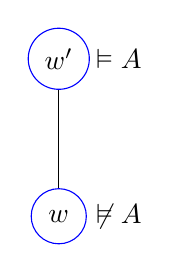
\begin{tikzpicture}
      \node [mstate] (1) at (0, 0) {$w'$};
      \node [right=10pt] at (1) {$\vDash A$};

      \node [mstate] (2) at (0, -2) {$w$};
      \node [right=10pt] at (2) {$\not\vDash A$};

      \draw (1) edge (2);
    \end{tikzpicture}
  \end{center}
\end{eg}

\begin{eg}
  This time consider the statement $w \vDash \neg \neg A \to A$. This takes some work to unravel.

  We need a world $w$ such that for all $w' \geq w$, if $w' \vDash \neg \neg A$, then $w' \vDash A$. If we unravel a bit more, we find that $w' \vDash \neg \neg A$ means for any $w'' \geq w'$, we can find some $w''' \geq w''$ such that $w''' \vDash A$.

  It is easy to see that actually in the model of the previous question, $w \not\vDash \neg \neg A \to A$, since $w \vDash \neg \neg A$, but $w \not\vDash A$.
\end{eg}

\begin{eg}
  The following model is a counter-model for $\neg \neg A \vee \neg A$:
  \begin{center}
    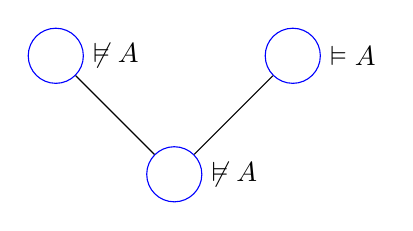
\begin{tikzpicture}
      \node [mstate] (b) at (0, 0) {};
      \node [right=10pt] at (b) {$\not\vDash A$};

      \node [mstate, above right=of b] (r) {};
      \node [right=10pt] at (r) {$\vDash A$};

      \node [mstate, above left=of b] (l) {};
      \node [right=10pt] at (l) {$\not\vDash A$};

      \draw (b) edge (r);
      \draw (b) edge (l);
    \end{tikzpicture}
  \end{center}
  where the bottom world believes in neither $\neg \neg A$ nor $\neg A$, since it sees worlds where $\neg A$ is true and also worlds where $A$ is true.
\end{eg}

Usually, we don't talk about a particular world believing in something. We talk about an entire structure of possible worlds believing something.
\begin{notation}
  If the root world of our model is $w$, then we write
  \[
    \vDash \varphi \Longleftrightarrow w \vDash \varphi.
  \]
\end{notation}
Almost by definition, if $\vDash \varphi$, then for any world $w'$, we have $w' \vDash \varphi$.

\begin{ex}
  Find a possible world model that does not believe Peirce's law.
\end{ex}

One can readily verify that classically, we have $(A \to B) \to B$ is equivalent to $A \vee B$, but they are not constructively equivalent.
\begin{ex}
  Find a possible world model that $\vDash (A \to B) \to B$, but does not $\vDash A \vee B$.
\end{ex}

\begin{ex}
  Find a possible world model that $\vDash (A \to B) \to B$ but does not believe $\vDash (B \to A) \to A$.
\end{ex}

\begin{ex}
  Find a possible world model that does not believe in $\vDash (A \to B) \vee (B \to A)$.
\end{ex}

Possible world semantics can be used for all sorts of logical systems, not just propositional logic. In general, the notion of accessibility need not be a partial order, but can be anything we want. Also, we do not necessarily have to require persistence. Of course, we also need to modify the according notion of a world.

\begin{eg}
  If we want to produce possible world semantics for constructive first-order logic, we need to modify our definition of worlds so that they have ``elements''. Assuming we have done so, we can encode $\forall$ and $\exists$ using the following rules:
  \begin{itemize}
    \item $w \vDash \exists_x, F(x)$ if there is some $y \in w$ for which $w \vDash F(y)$.
    \item $w \vDash \forall_x, F(x)$ if for all $w' \geq w$ and $x \in w'$, we have $w' \vDash F(x)$.
  \end{itemize}
  The second condition is much stronger than the naive ``for all $x \in w$, we have $w \vDash F(x)$'', because the $w'' \geq w$ may have many more elements. What our condition say is that $w$ somehow has a ``global'' way of showing that everything satisfies $F$.
\end{eg}

\begin{eg}
  The proposition $A \to \neg \neg A$ is valid all possible world models.

  % To see this, we note that if we have a world $w$ that believes in $A$, then by persistence, any world that $A$ sees also believes in $A$. We want to show that it does not believe in $\neg A$. % complete proof, make use of reflexivity and transitivity
\end{eg}

For classical logic, we had semantics given by truth tables. This easily shows that classical truth is decidable. Similarly, given any formula, it involves only finitely many variables, there are only finitely many distinct possible world models one has to check. So whether something is refuted by possible world models is again a decidable problem.

Now suppose we have a possible world model in front of us. Then given a formula $\varphi$, the set of worlds that believe $\varphi$ is an upward-closed subset of the frame. So we can think of the truth value of $\varphi$ as these upward-closed set.
\begin{eg}
  Suppose we have the following worlds:
  \begin{center}
    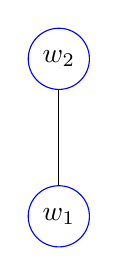
\begin{tikzpicture}
      \node [mstate] (1) at (0, 0) {$w_2$};

      \node [mstate] (2) at (0, -2) {$w_1$};

      \draw (1) edge (2);
    \end{tikzpicture}
  \end{center}
  Then the possible truth values are
  \[
    \emptyset, \{w_2\}, \{w_1, w_2\}.
  \]
  Suppose the top world believes $A$, but the bottom world does not. Then we say that $A$ has truth value $\{w_2\}$. This is indeed the three-valued algebra we used to disprove Peirce's law.
\end{eg}
What can we say about the collection of upward-closed subset of frames, i.e.\ our truth values? Under inclusion, it is easy to see that these are complete and co-complete, i.e.\ we have all infinite unions and intersections. More importantly, we can do ``implications''.
\begin{defi}[Heyting algebra]\index{Heyting algebra}
  A Heyting algebra is a poset with $\top$, $\bot$, $\wedge$ and $\vee$ and an operator $\Rightarrow$ such that $A \Rightarrow B$ is the largest $C$ such that
  \[
    C \wedge A \leq B.
  \]
\end{defi}
If a poset is complete co-complete, then we would expect the implication to be given by
\[
  A \Rightarrow B = \bigvee \{C : C \wedge A \leq B\}.
\]
Indeed, if the poset is a Heyting algebra, then it \emph{must} be given by this. So we just have to check that this works.

The thought is that Heyting algebras would ``validate'' all constructive theses, by interpreting $\wedge$ with $\wedge$, $\vee$ with $\vee$ and $\rightarrow$ with $\Rightarrow$. In other words, if we try to build a truth table for a formula with values in a Heyting algebra, we will get the top element $\top$ all the time iff the formula is constructively valid. So we have a parallel between the relation between classical logic and boolean algebras, and constructive logic and Heyting algebras.

It is an easy inductive proof that any constructively valid statement is ``true'' in all Heyting algebras, and the other direction is also true, but takes more work to prove.

Note that in classical logic, we only ever use the two-element boolean algebra. If we use the 4-element Boolean algebra, then we would detect the same set of tautologies. However, in the case of constructive logic we genuinely need all Heyting algebras.

Finally, we prove half the completeness theorem for possible world models.
\begin{lemma}
  Any formula with a natural deduction proof not using the rule for classical negation is true in all possible world models.
\end{lemma}
For any frame $F$, every such formula is satisfied by every possible world model on that frame. We say it is \emph{valid on $F$}. Such formulae are valid on all posets with a bottom element.

\begin{proof}
  The hard case is implication. Suppose we have a natural deduction proof of $A \to B$. The last rule is a $\to$-introduction. So by the induction hypothesis, every world that believes $A$ also believes $B$. Now let $w$ be a world that believes all the other undischarged assumptions in $A \to B$. By persistence, every $w' \geq w$ believes similarly. So any $w' \geq w$ that believes $A$ also believes $B$. So $w \vDash A \to B$.
\end{proof}

 % how about other half.

\subsection{Negative interpretation}
Suppose a constructive logician found a classical logician, and then they try to talk to each other. Then they would find that they disagree on a lot of things. The classical logician has no problems accepting $\neg \neg A \to A$, but the constructive logician thinks that is nonsense. Can they make sense of each other?

The classical logician can understand the constructive logician via possible world semantics. He could think that when the constructive logician says a proposition is false, they mean there are possible world models where the proposition fails. This is all fine.

But can a constructive logician make sense of the classical logician? When the constructivist sees $A \vee B$, he thinks that either we can prove $A$, or we can prove $B$. However, the classical logician views this as a much weaker statement. It is more a long the lines of ``it is not true that $A$ and $B$ are both false''. In general, we can try to interpret classical statements by putting in enough negations:
\begin{center}
  \begin{tabular}{cc}
    \toprule
    Classical proposition & Constructive interpretation\\
    \midrule
    $A \vee B$ & $\neg (\neg A \vee \neg B)$\\
    $A \wedge B$& $A \wedge B$\\
    $\exists_x W(x)$ & $\neg \forall_x \neg W(x)$\\
    $A \to B$ & $\neg (A \wedge \neg B)$\\
    \bottomrule
  \end{tabular}
\end{center}
This gives rise to the \emph{negative interpretation} of classical logic into constructive logic, due to G\"odel:
\begin{defi}[Negative interpretation]\index{negative interpretation}
  Given a proposition $\phi$, the interpretation $\phi^*$ is defined recursively by
  \begin{itemize}
    \item $\bot^* = \bot$.
    \item If $\varphi$ is atomic, then $\varphi^* = \neg\neg \varphi$.
    \item If $\varphi$ is negatomic, then $\varphi^* = \varphi$.
    \item If $\varphi = \psi \wedge \theta$, then $\varphi^* = \psi^* \wedge \theta^*$.
    \item If $\varphi = \psi \vee \theta$, then $\varphi^* = \neg (\neg \psi^* \wedge \neg \theta^*)$.
    \item If $\varphi = \forall_x \psi(x)$, then $(\forall_x)(\psi^*(x))$.
    \item If $\varphi = \psi \to \theta$, then $\varphi^* = \neg(\psi^* \wedge \neg \theta^*)$.
    \item If $\varphi = \exists_x \psi(x)$, then $\varphi^* = \neg \forall_x \neg \psi^*(x)$.
  \end{itemize}
\end{defi}
One can check that we always have $\vdash \varphi \to \varphi^*$. So the constructive version is always stronger.

\begin{defi}[Stable formula]\index{stable formula}
  A formula is \emph{stable} if
  \[
    \vdash \varphi^* \to \varphi.
  \]
\end{defi}

\begin{lemma}
  Any formula built up from negated and doubly negated atomics by $\neg$, $\wedge$ and $\forall$ is stable.
\end{lemma}

\begin{proof}
  By induction on formulae. The base case is immediate, using the fact that $\neg \neg \neg A \to \neg A$. This follows from the more general fact that
  \[
    (((p \to q) \to q) \to q) \to p \to q.
  \]
  It is less confusing to prove this in two steps, and we will write $\lambda$-terms for our proofs. First note that if we have $f: A \to B$, then we can obtain $f^T: (B \to q) \to A \to q$ for any $q$, using
  \[
    f^T = \lambda g_{B \to q}. \lambda a_A. g(f(a)).
  \]
  So it suffices to prove that
  \[
    p \to (p \to q) \to q,
  \]
  and the corresponding term is
  \[
    \lambda x_p. \lambda g_{p \to q}. g x
  \]
  We now proceed by induction.
  \begin{itemize}
    \item Now assume that we have proofs of $\neg \neg p \to p$ and $\neg \neg q \to q$. We want to prove $p \wedge q$ from $\neg \neg (p \wedge q)$. It suffices to prove $\neg \neg p$ and $\neg \neg q$ form $\neg \neg (p \wedge q)$, and we will just do the first one by symmetry.

      We suppose $\neg p$. Then we know $\neg (p \wedge q)$. But we know $\neg \neg (p \wedge q)$. So we obtain a contradiction. So we have proved that $\neg \neg p$.
    \item Note that we have
      \[
        \vdash \exists_x \neg \neg \varphi(x) \to \neg \neg \exists_x \varphi(x),
      \]
      but not the other way round. For universal quantification, we have
      \[
        \neg \neg \forall_x \varphi(x) \to \forall_x \neg \neg \varphi(x),
      \]
      but not the other way round. We can construct a proof as follows:
      \begin{prooftree}
        \AxiomC{$[\forall_x \varphi(x)]^1$}
        \elim{$\forall$}
        \UnaryInfC{$\varphi(a)$}
        \AxiomC{$[\neg \varphi(x)]^2$}
        \elim{$\to$}
        \BinaryInfC{$\to$}
        \intron{$\to$}{1}
        \UnaryInfC{$\neg \forall_x \varphi(x)$}
        \AxiomC{$[\neg \neg \forall_x \varphi(x)]^3$}
        \elim{$\to$}
        \BinaryInfC{$\bot$}
        \intron{$\to$}{2}
        \UnaryInfC{$\neg \neg \varphi(a)$}
        \intro{$\forall$}
        \UnaryInfC{$\neg \neg \forall_x \varphi(x)$}
        \intron{$\to$}{3}
        \UnaryInfC{$\neg \neg \forall_x F(x) \to \forall_x \neg \neg F(x)$}
      \end{prooftree}
      We now want to show that if $\varphi$ is stable, then $\forall_x \varphi(x)$ is stable. In other words, we want
      \[
        \neg \neg \forall_x \varphi^*(x) \to \forall_x \varphi^*(x).
      \]
      But form $\neg \neg \forall_x \varphi^*(x)$, we can deduce $\forall_x \neg \neg \varphi^*(x)$, which implies $\forall_x \varphi^* (x)$.
  \end{itemize}
  So every formula in the range of the negative interpretation is stable. Every stable formula is equivalent to its double negation (classically). Every formula is classically equivalent to a stable formula.
\end{proof}
So if a constructive logician meets a classical logician who is making some bizarre assertions about first order logic. To make sense of this, the constructive logician can translate it to its negative interpretation, which the classical logician thinks is equivalent to the original one.

\subsection{Constructive mathematics}
We now end with some remarks about how we can do mathematics ``constructively'', and the subtleties we have to be careful of.

We first discuss the notion of finiteness. Even classically, if we do not have the axiom of choice, then we have many distinct notions of ``finite set''. When we go constructive, things get more complicated.

We can produce (at least) two different definitions of finiteness.
\begin{defi}[Kuratowski finite]\index{Kuratowski finite}\index{finite!Kuratowski}
  We define ``finite'' recursively: $\emptyset$ is Kuratowski finite. If $x$ is Kuratowski finite, then so is $x \cup \{y\}$.
\end{defi}

There is a separate definition of $N$-finiteness:
\begin{defi}[$N$-finite]\index{$N$-finite}\index{finite!$N$}
  $\emptyset$ is $N$-finite. If $x$ is $N$-finite, and $y \not \in x$, then $x \cup \{y\}$ is $N$-finite.
\end{defi}
These two definitions are not the same! In a $N$-finite set, we know any two things are either equal, or they are not, as this is built into the definition of an $N$-finite set. However, in the case of Kuratowski finite, this is not true, since we don't have the law of excluded middle. We say $N$-finite sets have \term{decidable equality}.
If we want to do constructive arithmetic, the correct notion is $N$-finiteness.

We can still define natural numbers as the smallest set containing $\emptyset$ and is closed under successor. This gives us $N$-finite sets, but the least number principle is dodgy. It turns out the least number principle implies excluded middle.

There are also subtleties involving the notion of a non-empty set!
\begin{defi}[Non-empty set]\index{non-empty set}
  A set $x$ is \emph{non-empty} if $\neg \forall_yy \not \in x$.
\end{defi}

\begin{defi}[Inhabited set]\index{inhabited set}
  A set $x$ is \emph{inhabited} if $\exists_yy \in x$.
\end{defi}

They are not the same! Being inhabited is stronger than being non-empty! We shall not go into more details about constructive mathematics, because, disappointingly, very few people care.

\section{Model theory}

\subsection{Universal theories}
Recall the following definition:
\begin{defi}[Universal theory]\index{universal theory}
  A universal theory is a theory that can be axiomatized in a way such that all axioms are of the form
  \[
    \forall_{\cdots}(\text{stuff not involving quantifiers})\tag{$*$}
  \]
\end{defi}
For example, groups, rings, modules etc. are universal theories. It is easy to see that if we have a model of a universal theory, then any substructure is also a model.

It turns out the converse is also true! If a theory is such that every substructure of a model is a model, then it is universal. This is a very nice result, because it gives us a correspondence between syntax and semantics.

The proof isn't very hard, and this is the first result we will prove about model theory. We begin with some convenient definitions.
\begin{defi}[Diagram]\index{diagram}
  Let $\mathcal{L}$ be a language and $\mathcal{M}$ a structure of this language. The \emph{diagram} of $\mathcal{M}$ is the theory obtained by adding a constant symbol $a_x$ for each $x \in \mathcal{M}$, and then taking the axioms to be all quantifier-free sentences that are true in $M$. We will write the diagram as $D(\mathcal{M})$.
%
% The \emph{diagram} of a structure $\mathcal{M}$ is the theory obtained by expanding $\mathcal{M}$ by giving names to all its elements, and then recording all atomic truths about them.
\end{defi}
%
%\begin{defi}[Expansion and reduct of structure]\index{expansion of structure}\index{reduct of structure}
% The \emph{expansion} of a structure is what we get when we add more gadgets, i.e.\ add more things to the signature. A \emph{reduct} of a structure is what we get when we forget gadgets.
%\end{defi}
%Here we change the signature but not the carrier set.
%
%\begin{eg}
% $\bra \Q, 0, +, \leq\ket$ is an expansion of $\bra \Q, \leq\ket$. Conversely, $\bra \Q, \leq\ket$ is a reduct of $\bra \Q, 0, +, \leq \ket$.
%\end{eg}
%
%\begin{defi}[Extension and substructure]\index{extension}\index{substructure}
% An \emph{extension} of a structure is a superstructure of the same signature. A substructure is what you think it is.
%\end{defi}
%
%\begin{eg}
% $\bra \R, \leq\ket$ is an extension of $\bra \Q, \leq\ket$, and $\bra \Q, \leq\ket$ is a substructure of $\bra \R, \leq\ket$.
%\end{eg}

\begin{lemma}
  Let $T$ be a consistent theory, and let $T_{\forall}$ be the set of all universal consequences of $T$, i.e.\ all things provable from $T$ that are of the form $(*)$. Let $\mathcal{M}$ be a model of $T_\forall$. Then $T \cup D(\mathcal{M})$ is also consistent.
\end{lemma}

\begin{proof}
  Suppose $T \cup D(\mathcal{M})$ is not consistent. Then there is an inconsistency that can be derived from finitely many of the new axioms. Call this finite conjunction $\psi$. Then we have a proof of $\neg \psi$ from $T$. But $T$ knows nothing about the constants we added to $T$. So we know $T\vdash \forall_{\mathbf{x}} \neg \psi$. This is a universal consequence of $T$ that $\mathcal{M}$ does not satisfy, and this is a contradiction.
\end{proof}

\begin{thm}
  A theory $T$ is universal if and only if every substructure of a model of $T$ is a model of $T$.
\end{thm}

\begin{proof}
  $\Rightarrow$ is easy. For $\Rightarrow$, suppose $T$ is a theory such that every substructure of a model of $T$ is still a model of $T$.

  Let $\mathcal{M}$ be an arbitrary model of $T_\forall$. Then $T \cup D(\mathcal{M})$ is consistent. So it must have a model, say $\mathcal{M}^*$, and this is in particular a model of $T$. Moreover, $\mathcal{M}$ is a submodel of $\mathcal{M}^*$. So $\mathcal{M}$ is a model of $T$.

  So any model of $T_{\forall}$ is also a model of $T$, and the converse is clearly true. So we know $T_{\forall}$ is equivalent to $T$.
\end{proof}

\subsection{Products}
In model theory, we would often like to produce new models of a theory from old ones. One way to do so is via products.

We will use $\lambda$-notation to denote functions.
\begin{defi}[Product of structures]\index{product of structures}
  Suppose $\{A_i\}_{i \in I}$ is a family of structures of the same signature. Then the product
  \[
    \prod_{i \in I} A_i
  \]
  has carrier set the set of all functions
  \[
    \alpha: I \to \bigcup_{i \in I} A_i
  \]
  such that $\alpha(i) \in A_i$.

  Given an $n$-ary function $f$ in the language, the interpretation in the product is given pointwise by
  \[
    f(\alpha_1, \cdots, \alpha_n) = \lambda i. f(\alpha_1(i), \cdots, \alpha_n(i)).
  \]
  Relations are defined by
  \[
    \varphi(\alpha_1, \cdots, \alpha_n) = \bigwedge_{i \in I} \varphi(\alpha_1(i), \cdots, \alpha_n(i)).
  \]
\end{defi}
The natural question to ask is if we have a model of a theory, then is the product a model again? We know this is not always true. For example, the product of groups is a group, but the product of total orders is not a total order.

We say a product \emph{preserves} a formula $\varphi$ if
\[
  \prod_{i \in I} A_i \vDash \varphi \Longleftrightarrow \forall_{i \in I}, A_i \vDash \varphi
\]
What sort of things do products preserve? As we know from undergraduate mathematics, theories such as groups and rings are preserved.
\begin{defi}[Equational theory]\index{equational theory}
  An equational theory is a theory all of whose axioms are of the form
  \[
    \forall_{\mathbf{x}} (w_1(\mathbf{\mathbf{x}}) = w_2(\mathbf{x})),
  \]
  where $w_i$ are some terms in $\mathbf{x}$.
\end{defi}
It is not hard to see that models of equational theories are preserved under products.

It turns out actually the class of things preserved by products is much more general.

\begin{defi}[Horn clause]\index{Horn clause}
  A \emph{Horn clause} is a disjunction of atomics and negatomics of which at most one disjunct is atomic. % need a definition of negatomic somewhere

  It is usually better to think of Horn clauses as formulae of the form
  \[
    \left(\bigwedge \varphi_i\right) \to \chi
  \]
  where $\varphi_i$ and $\chi$ are atomic formulae. Note that $\bot$ is considered an atomic formula.

  A \term{universal Horn clause}\index{Horn clause!universal} is a universal quantifier followed by a Horn clause.
\end{defi}

\begin{eg}
  Transitivity, symmetry, antisymmetry, reflexivity are all universal Horn clauses.
\end{eg}

\begin{prop}
  Products preserve (universal) Horn formulae.
\end{prop}

\begin{proof}
  Suppose every factor
  \[
    A_i \vDash \forall_{\mathbf{x}} \bigwedge \varphi_i(\mathbf{x}) \to \chi(\mathbf{x}).
  \]
  We want to show that the product believes in the same statement. So let $(f_1, \cdots, f_k)$ be a tuple in the product of the right length satisfying the antecedent, i.e.\ for each $n \in I$, we have
  \[
    A_n \vDash \varphi_i (f_1(n), \cdots, f_k(n))
  \]
  for each $i$, But then by assumption,
  \[
    A_n \vDash \chi(f_1(n), \cdots, f_k(n))
  \]
  for all $n$. So the product also believes in $\varphi_j(f_1, \cdots, f_n)$. So we are done.
\end{proof}

\subsubsection*{Reduced products}
Unfortunately, it is rarely the case that products give us new interesting models. However, \emph{reduced} products do.

Reduced products arise from having a filter on the index set.
\begin{defi}[Filter]\index{filter}
  Let $I$ be a set. A \emph{filter} on $I$ is a (non-empty) subset $F \subseteq P(I)$ such that $F$ is closed under intersection and superset. A \term{proper filter}\index{proper filter}\index{filter!proper} is a filter $F \not= P(I)$.
\end{defi}

The intuition to hang on to is that $F$ captures the intuition of ``largeness''.
\begin{eg}
  Take $I = \N$, and $F$ the set of cofinite subsets of $\N$, namely the sets whose complement are finite, then $F$ is a filter.

  Similarly, we can take $F$ to contain the set of naturals with asymptotic density $1$.
\end{eg}

\begin{eg}
  Let
  \[
    F = \{x \subseteq \N: 17 \in \N\}
  \]
  Then this is a \emph{maximal} proper filter.
\end{eg}
This is a rather silly filter. We will see later that model-theoretically, these give us uninteresting reduced products.

\begin{defi}[Principal filter]\index{principal filter}
  A \emph{principal filter} is a filter of the form
  \[
    F = \{X \subseteq I: x \not\in X\}
  \]
  for some $x \in I$.
\end{defi}
We don't tend to care about principal filter, as they are boring.

\begin{defi}[Complete filter]\index{complete filter}\index{$\kappa$-complete filter}\index{filter!complete}\index{filter!$\kappa$-complete}
  A filter $F$ is $\kappa$-complete if it is closed under intersection of $<\kappa$ many things.
\end{defi}

\begin{eg}
  By definition, every filter is $\aleph_0$-complete.
\end{eg}

\begin{eg}
  Principal filters are $\kappa$-complete for all $\kappa$.
\end{eg}

A natural question is, are there any non-principal ultrafilters that are $\aleph_1$ complete? It turns out this is a deep question, and a lot of the study of set theory originated from this question.

Filters on $I$ form a complete poset under inclusion, with top element given by $F = P(I)$. Moreover, the \emph{proper} filters are a chain complete poset. Thus, by Zorn's lemma, there are \emph{maximal} proper filters.
\begin{defi}[Ultrafilter]\index{ultrafilter}
  An \emph{ultrafilter} is a maximal filter.
\end{defi}

We saw that principal filters are ultra. Are there non-principal ultrafilters? Fortunately, by Zorn's lemma, they do exist.
\begin{eg}
  By Zorn's lemma, there is a maximal filter extending the cofinite filter on $\N$, and this is non-principal.
\end{eg}
It turns out it is impossible to explicitly construct a non-principal ultrafilter, but Zorn's lemma says they exist.

%The dual notion to filter is an \term{ideal}, which are closed under union and subsets. They are called ideals because they are ideals in the corresponding boolean ring.

Now we can get to reduced products.
\begin{defi}[Reduced product]\index{reduced product}\index{product!reduced}
  let $\{A_i: i \in I\}$ be a family of structures, and $F$ a filter on $I$. We define the \emph{reduced product}
  \[
    \prod_{i \in I} A_i / F
  \]
  as follows: the underlying set is the usual product $\prod A_i$ quotiented by the equivalence relation
  \[
    \alpha \sim_F \beta \Longleftrightarrow \{i : \alpha(i) = \beta(i)\} \in F
  \]
  Given a function symbol $f$, the interpretation of $f$ in the reduced product is induced by that on the product.

  Given a relational symbol $\varphi$, we define
  \[
    \varphi(\alpha_1, \cdots, \alpha_n) \Longleftrightarrow \{i : \varphi(\alpha_1(i), \cdots, \alpha_n(i))\} \in F.
  \]
  If $F$ is an ultrafilter, then we call it the \term{ultraproduct}. If all the factors in an ultraproduct are the same, then we call it an \term{ultrapower}.
\end{defi}
It is an easy exercise to show that these are all well-defined. If we view the filter as telling us which subsets of $I$ are ``large'' then, our definition of reduced product says we regard two functions in the reduced products as equivalent if they agree on a ``large'' set.

Note that if our filter is principal, say $F = \{J \subseteq I: i \in J\}$, then the reduced product is just isomorphic to $A_i$ itself. So this is completely uninteresting.

%Suppose we have a family $\{A_i: i \in I\}$ of structures. We can as usual form the product $\prod A_i$. Suppose $F$ is a filter. Recall that $F$ is supposed to capture the notion of largeness. So we now form an equivalence relation on the elements by saying two elements are equal if they agree on a large set: For $f, g \in \prod A_i$, we say
%
%Observe that the definition of ``filter'' is designed to make $\sim_F$ an equivalence relation.
%
%\begin{defi}[Congruence relation]\index{congruence relation}
% We say an equivalence relation $\sim$ on $X$ is a \emph{congruence relation} for a function $f: X^m \to X$ iff for all $\mathbf{x}, \mathbf{y} \in X^m$ such that $x_i \sim y_i$ for all $i$, then
% \[
% f(\mathbf{x}) \sim f(\mathbf{y}).
% \]
%\end{defi}
%This in some sense says $f$ cannot tell equivalent things apart. Alternatively, this says $f$ passes on to a function $X^m/\sim \to X/\sim$.
%
%We can similarly define the notion of being a congruence relation for a predicate.
%\begin{eg}
% Equivalence mod $p$ is a congruence relation for $+$ and $\times$, but not for exponentiation.
%\end{eg}
%
%We now consider the quotient
%\[
% \prod_{i \in I} A_i/\sim_{F} = \prod_{i \in I} A_i /F.
%\]
%It is a very important, and also trivial, fact, that $\sim_F$ is a congruence relation for all the operations on the $A_i$ that are inherited by the product. The result is called the \term{reduced product} modulo $F$.

Reduced products preserve various things, but not everything. For example, the property of being a total order is in general not preserved by reduced products. So we still have the same problem.

But if the filter $F$ is an \emph{ultrafilter}, then nice things happen.

\begin{thm}[\L{}o\'s theorem]\index{\L{}o\'s theorem}
  Let $\{A_i: i \in I\}$ be a family of structures of the same (first-order) signature, and $\mathcal{U} \subseteq P(I)$ an ultrafilter. Then
  \[
    \prod_{i \in I} A_i/\mathcal{U} \vDash \varphi \Longleftrightarrow \{i: A_i \vDash \varphi\} \in \mathcal{U}.
  \]
  In particular, if $A_i$ are all models of some theory, then so is $\prod A_i / \mathcal{U}$.
\end{thm}

The key of the proof is the following lemma, which is a nice exercise:
\begin{lemma}
  Let $F$ be a filter on $I$. Then the following are equivalent:
  \begin{enumerate}
    \item $F$ is an ultrafilter.
    \item For $X \subseteq I$, either $X \in F$ or $I\setminus X \in F$ (``$F$ is prime'').
    \item If $X, Y \subseteq I$ and $X \cup Y \in I$, then $X \in I$ or $Y \in I$.
  \end{enumerate}
\end{lemma}
With this in mind, it is hard not to prove the theorem.

% How should we think about the elements of the ultraproduct? One can certainly view its elements as equivalence classes of elements in the product. However, sometimes it is helpful to think of the carrier set as the product itself, and instead weaken to notion of equality to say two things are equal if the are equivalent under $\sim_\mathcal{U}$.

%Note that there is an elementary embedding $K: \mathcal{M} \to \mathcal{M}^I/\mathcal{U}$ given by sending $m \in \mathcal{M}$ to $[\lambda i. m] \in \mathcal{M}^I/\mathcal{U}$.

%This is the natural inclusion one can think of, and we can show this is in fact elementary. It suffices to show that for any $m \in \mathcal{M}$, if there an $x \in \mathcal{M}^I/\mathcal{U}$ such that
%\[
% \mathcal{M}^I/\mathcal{U} \vDash \varphi(x, \iota(m)),
%\]
%then there is such an $x$ that is in the image of $\iota$.
%
%Consider such an $x$. It is an equivalence class of a family of functions which is almost everywhere related to $m$ by $\varphi$. So by \L{}o\'s theorem, tthere must be some $x' \in \mathcal{M}$ such that
%\[
% \mathcal{M} \vDash \varphi(x, m).
%\]
%Then we have
%\[
% \mathcal{M}^I/\mathcal{U} \vDash \varphi(\iota(x'), \iota(m')).
%\]
Let's now look at some applications of \L{}o\'s theorem.

Recall the compactness theorem of first order logic --- if we have a theory $T$ such that every finite subset of $T$ has a model, then so does $T$. The way we proved it was rather roundabout. We proved the completeness theorem of first order logic. Then we notice that if every finite subset of $T$ has a model, then every finite subset of $T$ is consistent. Since proofs are finite, we know $T$ is consistent. So by completeness, $T$ has a model.

Now that we are equipped with ultraproducts, it is possible to prove the compactness theorem directly!
\begin{thm}[Compactness theorem]\index{compactness theorem}
  Let $T$ be a theory in first order logic such that every finite subset has a model. Then $T$ has a model.
\end{thm}

\begin{proof}
  Let $\Delta$ be such a theory. Let $S = \mathcal{P}_{\aleph_0}(\Delta)$ be the set of all finite subsets of $\Delta$. For each $s \in S$, we pick a model $\mathcal{M}_s$ of $s$.

  Given $s \in S$, we define
  \[
    X_s = \{t \in S: s \subseteq t\}.
  \]
  We notice that $\{X_s: s \in S\}$ generate a proper filter on $S$. We extend this to ultrafilter $\mathcal{U}$ by Zorn's lemma. Then we claim that
  \[
    \prod_{s \in S} \mathcal{M}_s/\mathcal{U}\vDash \Delta.
  \]
  Indeed, for any $\varphi \in \Delta$, we have
% To see this, we note that for any $\varphi \in \Delta$, we have $X_{\{\varphi\}} \in \mathcal{U}$. Also, for any $s \in X_{\{\varphi\}}$, we have $\mathcal{M}_s \vDash \varphi$. So
  \[
    \{s: \mathcal{M}_s \vDash \varphi\} \supseteq X_{\{\varphi\}} \in \mathcal{U}.
  \]
\end{proof}

\begin{eg}
  Let $T$ be the theory consisting of all first-order statements true in $\bra \R, 0, 1, +, \times\ket$. Add to $T$ a constant $\varepsilon$ and the axioms $\varepsilon < \frac{1}{n}$ for all $n \in \N$. Then for any finite subset of this new theory, $\R$ is still a model, by picking $\varepsilon$ small enough. So by the compactness theorem, we know this is consistent.

  Using \emph{our} proof of the compactness theorem, we now have a ``concrete'' model of real numbers with infinitesimals --- we just take the ultraproduct of infinitely many copies of $\R$.
\end{eg}

\subsection{Ehrenfeucht--Mostowski theorem}
\begin{defi}[Skolem function]\index{Skolem function}
  \emph{Skolem functions} for a structure are functions $f_\varphi$ for each $\varphi \in \mathcal{L}$ such that if
  \[
    \mathcal{M} \vDash \forall_\mathbf{x} \exists_\mathbf{y} \varphi(\mathbf{x}, \mathbf{y}),
  \]
  then
  \[
    \mathcal{M} \vDash \forall_\mathbf{x} \varphi(\mathbf{x}, f_\varphi(\mathbf{x})).
  \]
\end{defi}

\begin{defi}[Skolem hull]\index{Skolem hull}
  The \emph{Skolem hull} of a structure is obtained from the constants term by closure under the Skolem functions.
\end{defi}

\begin{defi}[Elementary embedding]\index{elementary embedding}
  Let $\Gamma$ be a set of formulae. A function $i: \mathcal{M}_1 \to \mathcal{M}_2$ is \term{$\Gamma$-elementary} iff for all $\varphi \in \Gamma$ we have $\mathcal{M}_1 \vDash \varphi(\mathbf{x})$ implies $\mathcal{M}_2 \vDash \varphi(i(\mathbf{x}))$.

  If $\Gamma$ is the set of all formulae in the language, then we just say it is \emph{elementary}.
\end{defi}
Usually, we take $\Gamma$ to be the set of all formulae, and $\mathcal{M}_1$ to be a substructure of $\mathcal{M}_2$.

\begin{eg}
  It is, at least intuitively, clear that the inclusion $\bra \Q, \leq\ket \hookrightarrow \bra \R, \leq \ket$ is elementary.

  However, $\Q$ as a field is \emph{not} elementary as a substructure of $\R$ as a field.
\end{eg}

Note that first order logic is not decidable. However, \emph{monadic} first order logic is.
\begin{defi}[Monadic first order logic]\index{monadic first order logic}\index{first order logic!monadic}
  \emph{Monadic first-order logic} is first order logic with only one-place predicates, no equality and no function symbols.
\end{defi}

\begin{prop}
  Monadic first-order logic is decidable.
\end{prop}

\begin{proof}
  Consider any formula $\varphi$. Suppose it involves the one-place predicates $p_1, \dots, p_n$. Given any structure $\mathcal{M}$, we consider the quotient of $\mathcal{M}$ by
  \[
    x \sim y \Leftrightarrow p_i (x) = p_i(y) \text{ for all i}.
  \]
  Then there are at most $2^n$ things in the quotient.

  Then given any transversal of the quotient, we only have to check if the formula holds for this transversal, and this is finite. So we can decide.
\end{proof}

\begin{defi}[Set of indiscernibles]\index{set of indiscernibles}
  We say $\bra I, \leq_I\ket$ is a \emph{set of indiscernibles} for $\mathcal{L}$ and a structure $\mathcal{M}$ with $I \subseteq \mathcal{M}$ if for any $\varphi \in \mathcal{L}(M)$ of arity $n$, and for all increasing tuples $\mathbf{x}, \mathbf{y} \in I$,
  \[
    \mathcal{M} \vDash \varphi(\mathbf{x}) \Longleftrightarrow \mathcal{M} \vDash \varphi(\mathbf{y})
  \]
\end{defi}
This is weaker than just saying everything in there are the same.

\begin{eg}
  $\bra \Q, I\ket$ is a set of indiscernibles for $\bra \R, \leq\ket$.
\end{eg}

Let $T$ be a theory with infinite models. The general line of thought is --- can we get a model of $T$ with special properties?

Given any set $\mathcal{M}$, invent names for every member of $\mathcal{M}$. Add these names to the language of $T$. We add axioms to say all these constants are distinct. Since $T$ has infinite models, we know this theory has a model.

Let $\Omega$ be the set of countable ordinals, consider the language of $\R$, and add a name to this language for every countable ordinal. We further add axioms to say that $\alpha < \beta$ in the ordering of $\R$ whenever $\alpha < \beta$ as ordinals.

Again by compactness, we find that this has a model. So we can embed the set of countable ordinals into a model of reals, which we know is impossible for the genuine $\R$. However, in general, there is no reason to believe these elements are a set of indiscernibles. What Ehrenfeucht--Mostowski says is that we can in fact do so.

\begin{thm}[Ehrenfeucht--Mostowski theorem (1956)]\index{Ehrenfeucht--Mostowski theorem}
  Let $\bra I, \leq\ket$ be a total order, and let $T$ be a theory with infinite models. Suppose we have a unary predicate $P$ and a $2$-ary relation $\preccurlyeq \in \mathcal{L}(T)$ such that
  \[
    T \vdash \text{$\preccurlyeq$ is a total order on $\{x: P(x)\}$}.
  \]
  Then $T$ has a model $\mathcal{M}$ with a copy of $I$ as a sub-order of $\preccurlyeq$, and the copy of $I$ is a set of indiscernibles. Moreover, we can pick $\mathcal{M}$ such that every order-automorphism of $\bra I, \leq \ket$ extends to an automorphism of $\mathcal{M}$.
\end{thm}

We will give two proofs of this result. We first give the original proof of Ehrenfeucht--Mostowski, which uses Ramsey theory.
\begin{proof}
  Let $T$ and $\bra I, \leq \ket$ be as in the statement of the theorem. We add to $\mathcal{L}(T)$ names for every element of $I$, say $\{c_i: i \in I\}$. We add axioms that says $P(c_i)$ and $c_i \preccurlyeq c_j$ whenever $i < j$. We will thereby confuse the orders $\leq$ and $\preccurlyeq$, partly because $\leq$ is much easier to type. We call this theory $T^*$.

  Now we add to $T^*$ new axioms to say that the $c_i$ form a set of indiscernibles. So we are adding axioms like
  \[
    \varphi(c_i, c_j) \Leftrightarrow \varphi(c_{i'}, c_{j'})\tag{$*$}
  \]
  for all $i < j$ and $i' < j'$. We do this simultaneously for all $\varphi \in \mathcal{L}(T)$ and all tuples of the appropriate length. We call this theory $T^I$, and it will say that $\bra I, \leq\ket$ forms a set of indiscernibles. The next stage is, of course, to prove that $T^I$ is consistent.

  Consider any finite fragment $T'$ of $T^I$. We want to show that $T'$ is consistent. By finiteness, $T'$ only mentions finitely many constants, say $c_1 < \cdots < c_K$, and only involve finitely many axioms of the form $(*)$. Denote those predicates as $\varphi_1, \cdots, \varphi_n$. We let $N$ be the supremum of the arities of the $\varphi_i$.

  Pick an infinite model $\mathcal{M}$ of $T$. We write
  \[
    \mathcal{M}^{[N]} = \{A \subseteq \mathcal{M}: |A| = N\},
  \]
  For each $\varphi_i$, we partition $\mathcal{M}^{[N]}$ as follows --- given any collection $\{a_k\}_{k = 1}^N$, we use the order relation $\preccurlyeq$ to order them, so we suppose $a_k \preccurlyeq a_{k + 1}$. If $\varphi_i$ has arity $m \leq N$, then we can check whether $\varphi_i(a_1, \cdots, a_m)$ holds, and the truth value gives us a partition of $\mathcal{M}^{[N]}$ into 2 bits.

  If we do this for all $\varphi_i$, then we have finitely partitioned $\mathcal{M}^{[N]}$. By Ramsey's theorem, this has an infinite monochromatic subset, i.e.\ a subset such that any two collection of $N$ members fall in the same partition. We pick elements $c_1, \cdots, c_K, \cdots, c_{K + N}$, in increasing order (under $\preccurlyeq$). We claim that picking the $c_1, \cdots, c_K$ to be our constants satisfy the axioms of $T'$.

  Indeed, given any $\varphi_i$ mentioned in $T'$ with arity $m < N$, and sequences $c_{\ell_1} < \cdots < c_{\ell_m}$ and $c_{\ell_1'} < \cdots < c_{\ell_m'}$, we can extend these sequences on the right by adding more of those $c_i$. Then by our choice of the colouring, we know
  \[
    \varphi_i(c_{\ell_1}, \cdots, c_{\ell_m}) \Leftrightarrow \varphi_i(c_{\ell_1'}, \cdots, _{\ell_m'}).
  \]
  So we know $T'$ is consistent. So $T^I$ is consistent. So we can just take a model of $T^I$, and the Skolem hull of the indiscernibles is the model desired.
\end{proof}

There is another proof of Ehrenfeucht--Mostowski due to Gaifman, using ultraproducts. We will sketch the proof here.

To do so, we need the notion of colimits.
\begin{defi}[Colimit]\index{colimit}
  Let $\{A_i: i \in I\}$ be a family of structures index by a poset $\bra I, \leq\ket$, with a family of (structure-preserving) maps $\{\sigma_{ij}: A_i \hookrightarrow A_j \mid i \leq j\}$ such that whenever $i \leq j \leq k$, we have
  \[
    \sigma_{jk} \sigma_{ij} = \sigma_{ik}.
  \]
  In particular $\sigma_{ii}$ is the identity. A \emph{colimit} or \term{direct limit} of this family of structures is a ``minimal'' structure $A_\infty$ with maps $\sigma_i: A_i \hookrightarrow A_\infty$ such that whenever $i \leq j$, then the maps
  \[
    \begin{tikzcd}
      A_i \ar[d, "\sigma_{ij}"'] \ar[r, "\sigma_i"] & A_\infty\\
      A_j \ar[ur, "\sigma_j"']
    \end{tikzcd}
  \]
  commute.

  By ``minimal'', we mean if $A_\infty'$ is another structure with this property, then there is a unique inclusion map $A_\infty \hookrightarrow A_\infty'$ such that for any $i \in I$, the maps
  \[
    \begin{tikzcd}
      A_i \ar[r, "\sigma_i"] \ar[rd, "\sigma_i'"'] & A_\infty\ar[d, hook]\\
      & A_\infty'
    \end{tikzcd}
  \]
\end{defi}

\begin{eg}
  The colimit of a family of sets is obtained by taking the union of all of them, and then identifying $x \sim \sigma_{ij}(x)$ for all $x \in A_i$ and $i \leq j$.
\end{eg}

The key observation is the following:
\begin{significant}
  Every structure is a direct limit of its finitely generated substructures, with the maps given by inclusion.
\end{significant}
We will neither prove this nor make this more precise, but it will be true for the different kinds of structures we are interested in. In particular, for a poset, a finitely generated substructure is just a finite suborder, because there are no function symbols to ``generate'' anything in the language of posets.

To prove Ehrenfeucht--Mostowski, we construct a model satisfying the statement of Ehrenfeucht--Mostowski as the direct limit of structures indexed by finite subset of $I$:
\[
  \{\mathcal{M}_s: s \in \mathcal{P}(I)\}
\]
and when $s \subseteq t \in \mathcal{P}(I)$, we have an elementary embedding $\mathcal{M}_s \hookrightarrow \mathcal{M}_t$. We then note that if all the $\sigma_{ij}$ are elementary, then the $\sigma_i: A_i \hookrightarrow A_\infty$ are also elementary. In particular, if each $\mathcal{M}_s$ are models of our theory, then so is $A_\infty$.

We start by picking any infinite model $\mathcal{M}$ of $I$. By standard compactness arguments, we may wlog there is no last $\preccurlyeq$-thing in $\mathcal{M}$, and also that $J = \{x: P(x)\}$ is infinite. We pick $\mathcal{U}$ an ultrafilter on $J$ that contains all terminal segments of $\preccurlyeq$. Since $J$ does not have a last element, this is a non-principal ultrafilter.

We now write
\[
  L(\mathcal{M}) = \mathcal{M}^{|J|}/\mathcal{U}.
\]
We will define
\[
  \mathcal{M}_s = L^{|s|}(\mathcal{M}).
\]
In particular, $\mathcal{M}_{\emptyset} = \mathcal{M}$.

To construct the embedding, we consider the following two classes of maps:
\begin{enumerate}
  \item For any structure $\mathcal{M}$, there is a map $K = K(\mathcal{M}): \mathcal{M} \to L(\mathcal{M})$ given by the constant embedding.
  \item If $i$ is an embedding from $\mathcal{M}$ into $\mathcal{N}$, then there is an embedding
    \[
      L(i): L(\mathcal{M}) \to L(\mathcal{N}).
    \]
    which is ``compose with $i$ on the right''.
\end{enumerate}
It is easy to see that both of these maps are elementary embeddings, where we require $i$ to be elementary in the second case. Moreover, these maps are compatible in the sense that the following diagram always commutes:
\[
  \begin{tikzcd}
    \mathcal{M} \ar[r, "i"] \ar[d, "K(\mathcal{M})"] & \mathcal{N} \ar[d, "K(\mathcal{N})"]\\
    L(\mathcal{M}) \ar[r, "L(i)"'] & L(\mathcal{N})
  \end{tikzcd}
\]
%How do we construct these $\mathcal{M}_s$? We start with any model $\mathcal{M}$ of $T$. We are going to assume that there is no last $\preccurlyeq$-thing in $\mathcal{M}$, and also that the graph of $\preccurlyeq$ is infinite. We let $\mathcal{U}$ be a non-principal ultrafilter $J = \{x: P(x)\}$. Then we pick $\mathcal{M}_s$ to be the result of doing an ultrapower construction using $\mathcal{U}$, $|s|$ many times to $\mathcal{M}$. The tricky bit is to construct the embeddings.
%We define this by recursion. We write $\last(s)$ for the last element of $s$, and $\butlast(s)$ for $s \setminus \{\last(s)\}$. Given a structure $\mathcal{M}$, we write
%\[
% L(\mathcal{M}) = \mathcal{M}^p/\mathcal{U}.
%\]
%We need two gadgets
%\begin{enumerate}
% \item An elementary embedding $K(\mathcal{M}): \mathcal{M} \to L(\mathcal{M})$.
% \item If $i$ is an embedding from $\mathcal{M}$ into $\mathcal{N}$, then there is an
% \[
% L(i): L(\mathcal{M}) \to L(\mathcal{N}).
% \]
% which is ``compose with $i$ on the right''.
%\end{enumerate}
%Moreover, these are compatible in the sense
%\[
% \begin{tikzcd}
% \mathcal{M} \ar[r, "i"] \ar[d, "K(\mathcal{M})"] & \mathcal{N} \ar[d, "K(\mathcal{N})"]\\
% L(\mathcal{M}) \ar[r, "L(i)"] & L(\mathcal{N})
% \end{tikzcd}
%\]
%We can now recursively define $I(s, t): \mathcal{M}_s \to \mathcal{M}_t$.
We now further consider the functions $\head$ and $\tail$ defined on finite linear orders by
\begin{align*}
  \head(a_1 < \cdots < a_n) &= a_1\\
  \tail(a_1 < \cdots < a_n) &= a_2 < \cdots < a_n.
\end{align*}
We can now define the embeddings recursively. We write $I(s, t)$ for the desired inclusion from $\mathcal{M}_s$ into $\mathcal{M}_t$. We set
\begin{itemize}
  \item If $s = t$, then $I(s, t)$ is the identity.
  \item If $\head(s) = \head(t)$, then $I(s, t)$ is $L(I(\tail(s), \tail(t)))$.
  \item Otherwise, $I(s, t)$ is $K \circ I(s, \tail(t))$.
% \item If $s = t$, then $I(s, t)$ is the identity.
% \item If $\last(s) = \last(t)$, then $I(s, t)$ is $L(I(\butlast(s), \butlast(t)))$. Otherwise, it is $K \circ I(s, \butlast(t))$.
\end{itemize}
By our previous remark, we know these are all elementary embeddings, and that these maps form a commuting set. Thus, we obtain a direct limit $\mathcal{M}_\infty$.

Now we want to produce a copy of $I$ in the direct limit. So we want to produce a copy of $s$ in $\mathcal{M}_s$ for each $s$, such that the maps preserve these copies. It suffices to be able to do it in the case $|s| = 2$, and then we can bootstrap it up by induction, since if $|s| > 3$, then we find two sets of $s$ of order $< |s|$ whose union gives $s$, and compatibility means we can glue them together. To ensure compatibility, we pick a fixed element $x \in L(\mathcal{M})$, and set this as the desired element in $\mathcal{M}_s$ whenever $|s| = 1$. It then suffices to prove that, say, if $0 < 1$, then $I(\{0\}, \{0, 1\})(x) < I(\{1\}, \{0, 1\})(x)$. It is then a straightforward exercise to check that
\[
  x = [\lambda p. p] \in L(\mathcal{M}) = \mathcal{M}^{|P|}/\mathcal{U}
\]
works.

Once we have done this, it is immediate that the copy of $I$ in the direct limit is a family of indiscernibles. Indeed, we simply have to check that the copy of $s$ in $\mathcal{M}_s$ is a family of indiscernibles, since every formula only involves finitely many things. Then since the inclusino of $\mathcal{M}_s$ into $\mathcal{M}$ is elementary, the result follows..

%
%We construct this by induction. If $|s| = 1$, then $\mathcal{M}_s \cong \mathcal{M}$. We arbitrarily pick some $p \in \mathcal{M}$ and let it be our designated member.
%
%Now suppose know how to point to $|s|$-many things in $\mathcal{M}_s$. How about $\mathcal{M}_t$, where $|t| = |s| + 1$? We let $t'$ be $T$ with the penultimate elemenet deleted. By induction hypothesis, we know what the lsat thing in $\mathcal{M}_{t'}$ is. We have the embedding
%\[
% I(t', t): \mathcal{M}_{t'} \to \mathcal{M}_t.
%\]
%This will tells us which thing in the $|t|$th ultrapower is the designated element. % figure this out.
%
%Since every finite formula contains only finitely many constants, it follows that the copy of $I$ in the direct limit is a family of indiscernibles.

\subsection{The omitting type theorem}
\begin{defi}[Type]\index{type}\index{$n$-types}
  A \emph{type} is a set of formulae all with the same number of free variables. An \emph{$n$-type} is a set of formulae each with $n$ free variables.
\end{defi}
What is the motivation of this? A $1$-type is a set of formulae all with one free variable. So if we have a model $\mathcal{M}$ and an element $x \in \mathcal{M}$, then we can consider all formulae that $x$ satisfies, and we see that this gives as a $1$-type.

\begin{defi}[Realization of type]\index{realization of type}
  A model $\mathcal{M}$ \emph{realizes an $n$-type $\Sigma$} if there exists $x_1, \cdots, x_n \in \mathcal{M}$ such that for all $\sigma \in \Sigma$, we have
  \[
    \mathcal{M} \vDash \sigma(x_1, \cdots, x_n).
  \]
\end{defi}
%
%\begin{defi}[Saturated model]\index{saturated model}\index{model!saturated}\index{model!countably saturated}\index{$\aleph_0$-saturated model}\index{countably saturated model}
% We say a model $\mathcal{M}$ is called $\aleph_0$-saturated if $\mathcal{M}$ realizes every finitely satisfiable type.
%\end{defi}

Any fool can realize a type, but it takes a model theorist to omit one!

\begin{defi}[Omit a type]\index{omit a type}
  A model $\mathcal{M}$ \emph{omits an $n$-type $\Sigma$} if for all $x_1, \cdots, x_n$, there exists $\sigma \in \Sigma$ such that
  \[
    \mathcal{M} \not\vDash \sigma(x_1, \cdots, x_n).
  \]
\end{defi}

\begin{eg}
  Consider the language of PA, and consider the type containing $\sigma_i(x)$ saying $x \not= s^i(x)$. We really want to omit this type!

  Of course, it is not hard in this case --- the standard model of PA does.
\end{eg}

Let's look for a condition on $T$ and $\Sigma$ for $T$ to have a model that omits this type.

\begin{defi}[Locally realize]\index{locally realize a type}\index{realize a type!locally}
  We say $\varphi$ realizes $\Sigma$ locally if
  \[
    T \vdash \forall_x(\varphi(x) \to \sigma(x)).
  \]
\end{defi}
Suppose there is some $\varphi \in \mathcal{L}(T)$ such that
\[
  T \vdash \exists_x \varphi(x)
\]
and $\varphi(x)$ locally realizes $\Sigma$, then we certainly cannot omit $\Sigma$.

Now if $T \vDash \forall_x \neg \varphi(x)$ whenever $\varphi$ locally realizes $\Sigma$, then we have a chance. We say \term{$T$ locally omits $\Sigma$}. It turns out this is sufficient!

\begin{thm}[Omitting type theorem]\index{omitting type theorem}\index{type}
  Let $T$ be a first-order theory, and $\Sigma$ an $n$-type. If
  \[
    T \vdash \forall_x \neg \varphi(x)
  \]
  whenever $\varphi$ locally realizes $\Sigma$, then $T$ has a model omitting $\Sigma$.
\end{thm}

We first prove a special case for propositional logic.
\begin{thm}
  Let $T$ be a propositional theory, and $\Sigma \subseteq \mathcal{L}(T)$ a type (with $n = 0$). If $T$ locally omits $\Sigma$, then there is a $T$-valuation that omits $\Sigma$.
\end{thm}

\begin{proof}
  Suppose there is no $T$-valuation omitting $\Sigma$. By the completeness theorem, we know everything in $\Sigma$ is a theorem of $T$. So $T$ can't locally omit $\Sigma$.
\end{proof}
That was pretty trivial. But we can do something more than that --- the \emph{extended} omitting types theorem. It says we can omit countably many types simultaneously.

%\begin{thm}
% Let $T$ be a first-order theory, and for each $i \in \N$, we have a type $\Sigma_i$. If $T$ locally emits $\Sigma_i$ for all $i$, then $T$ has a model that omits every $\Sigma_i$.
%\end{thm}
%
%Again, we prove the propositional version first.
\begin{thm}
  Let $T$ be a propositional theory, and for each $i \in \N$, we let $\Sigma_i \subseteq \mathcal{L}(T)$ be types for each $i \in \N$. If $T$ locally omits each $\Sigma_i$, then there is a $T$-valuation omitting all $\Sigma_i$.
\end{thm}

\begin{proof}
  We will show that whenever $T \cup \{\neg A_1, \cdots, \neg A_i\}$ is consistent, where $A_n \in \Sigma_n$ for $n \leq i$, then we can find $A_{n + 1} \in \Sigma_{n + 1}$ such that
  \[
    T \cup \{\neg A_1, \cdots, \neg A_n, \neg A_{n + 1}\}
  \]
  is consistent.

  Suppose we can't do this. Then we know that
  \[
    T \vdash \left(\bigwedge_{1 \leq j \leq n} \neg A_j \right) \to A_{n + 1},
  \]
  for every $A_{n + 1} \in \Sigma_{n + 1}$. But by assumption, $T$ locally omits $\Sigma_{i + 1}$. This implies
  \[
    T \vdash \neg \left(\bigwedge_{1 \leq j \leq n} \neg A_j \right),
  \]
  contradicting the inductive hypothesis that $T \cup \{\neg A_1, \cdots, \neg A_i\}$ is consistent.

  Thus by compactness, we know $T \cup \{\neg A_1, \neg A_2, \cdots\}$ is consistent, and a model of this would give us a model of $T$ omitting all those types.
\end{proof}

We now prove the general case.
\begin{proof}
  Let $T$ be a first order theory (in a countable language) locally omitting $\Sigma$. For simplicity, we suppose $\Sigma$ is a $1$-type. We want to find a model omitting $\Sigma$. Suppose $T$ locally omits $\Sigma$, and let $\{c_i: i \in \N\}$ be a countable set of new constant symbols. Let $\bra \varphi_i: i \in \N\ket$ be an enumeration of the sentences of $\mathcal{L}(T)$. We will construct an increasing sequence $\{ T_i: i \in \N\}$ of finite extensions of $T$ such that for each $m \in \N$,
  \begin{enumerate}
    \item[(0)] $T_{m + 1}$ is consistent.
    \item $T_{m + 1}$ decides $\varphi_n$ for $n \leq m$, i.e.\ $T_{m + 1} \vdash \varphi_n$ or $T_{m + 1} \vdash \neg \varphi_n$.
    \item If $\varphi_m$ is $\exists_x \psi(x)$ and $\varphi_m \in T_{m + 1}$, then $\psi(c_p) \in T_{m + 1}$, where $c_p$ is the first constant not occurring in $T_m$ or $\varphi_m$.
    \item There is a formula $\sigma(x) \in \Sigma$ such that $\neg \sigma(c_m) \in T_{m + 1}$.
  \end{enumerate}
  We will construct this sequence by recursion. Given $T_m$, we construct $T_{m + 1}$ as follows: think of $T_m$ as $T \cup \{\theta_1, \cdots, \theta_r\}$, and let
  \[
    \Theta = \bigwedge_{j \leq r} \theta_j.
  \]
  We let $\{c_1, \cdots, c_N\}$ be the constants that have appeared in $\Theta$, and let
  \[
    \Theta(\mathbf{x})
  \]
  be the result of replacing $c_i$ with $x_i$ in $\theta$. Then clearly, $\Theta(\mathbf{x})$ is consistent with $T$. Since $T$ locally omits $\Sigma$, we know there exists some $\sigma(x) \in \Sigma$ such that
  \[
    \Theta \wedge \neg \sigma(x_m)
  \]
  is consistent with $T$. We put $\neg \sigma(c_m)$ into $T_{m + 1}$, and this takes care of (iii).

  If $\varphi_m$ is consistent with $T_m \cup \{\neg \sigma(c_m)\}$, then put it into $T_{m + 1}$. Otherwise, put in $\neg \varphi_m$. This takes care of (i).

  If $\varphi_m$ is $\exists_x \psi(x)$ and it's consistent with $T_m \cup \{\neg \sigma(c_m)\}$, we put $\psi(c_m)$ into $T_{m + 1}$. This takes care of (ii).

  Now consider
  \[
    T^* = \bigcup_{n \in \N} T_n
  \]
  Then $T^*$ is complete by construction, and is complete by compactness.

  Consider an arbitrary countable model of $T^*$, and the submodel generated by the constants in $C$. This is a model of $T^* \supseteq T$ and condition (iii) ensures that it omits $\Sigma$.
\end{proof}

\section{Computability theory}
\subsection{Computability}
We begin by discussing some number theory. Consider the Diophantine equation
\[
  x^2 + y^2 = z^2.\tag{$*$}
\]
We can certainly write down some solutions to this equation, e.g.
\[
  3^2 + 4^2 = 5^2.
\]
But is it possible to find \emph{all} solutions? It is a well-known result that we can. Of course, to do so, it suffices to enumerate all solutions where $x, y, z$ are coprime It turns out every such solution of $(*)$ can be written as
\[
  x = m^2 - n^2,\quad y = 2mn, z = m^2 + n^2
\]
for some $m, n \in \N$, and conversely, for any $m, n \in \N$, the $(x, y, z)$ given by this formula is a solution. Thus, if we want to list all solutions to $(*)$, then it suffices to plug in all possible values of $m$ and $n$. In other words, we have an \emph{algorithm} that enumerates all solutions to $(*)$.

Given any Diophantine equation, it would be great to have some similar algorithm that enumerates all solutions to the equation. But even before that, it would be great to have some algorithms that tell us whether there is any solution at all. This was Hilbert's 10th problem --- is there an algorithm that determines whether or not a Diophantine equation has a solution?

If such an algorithm existed, then to prove this, we merely have to exhibit such an algorithm, and prove that it works? But how could we prove that there \emph{isn't} one. To do so, we must formulate an ``algorithm'' as a \emph{mathematical object}. Alternatively, we want a formal notion of what is a ``computable'' function.

One way to do so is to define ``computable functions'' recursively. We will be concerned with functions $\N^n \to \N^m$ for different $k$ and $m$, and the idea is to list some functions that any sensible computer should be able to compute, and then close it under operations that really should preserve computability. We then hope that the set of functions produced this way is exactly the functions that can be ``computed'' by an ``algorithm''.

We start with a naive attempt, and what we obtain is known as ``primitive recursive'' functions.
\begin{defi}[Primitive recursive functions]\index{primitive recursive function}
  The class of \emph{primitive recursive functions} $\N^n \to \N^m$ for all $n, m$ is defined inductively as follows:
  \begin{itemize}
    \item The constantly zero function $f(\mathbf{x}) = 0$, $f: \N^n \to \N$ is primitive recursive.
    \item The successor function $\succ: \N \to \N$ sending a natural number to its successor (i.e.\ it ``plus one'') is primitive recursive.
    \item The identity function $\cid: \N \to \N$ is primitive recursive.
    \item The projection functions
      \[
        \begin{tikzcd}[cdmap]
          \proj_j^i (\mathbf{x}) : \N^j \ar[r] & \N\\
          (x_1, \cdots, x_j) \ar[r, maps to ]& x_i
        \end{tikzcd}
      \]
      are primitive recursive.
  \end{itemize}
  Moreover,
  \begin{itemize}
    \item Let $f: \N^k \to \N^m$ and $g_1, \cdots, g_k: \N^n \to \N$ be primitive recursive. Then the function
      \[
        (x_1, \cdots, x_n) \mapsto f(g_1(x_1, \cdots, x_n), \cdots, g_k(x_1, \cdots, x_n)): \N^n \to \N^m
      \]
      is primitive recursive.
  \end{itemize}
  Finally, we have closure under \term{primitive recursion}
  \begin{itemize}
    \item If $g: \N^k \to \N^m$ and $f: \N^{m + k + 1} \to \N^m$ are primitive recursive, then so is the function $h: \N^{k + 1} \to \N^m$ defined by
      \begin{align*}
        h(0, \mathbf{x}) &= g(\mathbf{x})\\
        h(\succ \; n, \mathbf{x}) &= f(h(n, \mathbf{x}), n, \mathbf{x}).
      \end{align*}
  \end{itemize}
\end{defi}
Do these give us everything we want? We first notice that we can define basic arithmetic using primitive recursion by
\begin{align*}
  \plus(0, n) &= n\\
  \plus(\succ\; m, n) &= \succ (\plus(m, n))\\
  \mult(1, n) &= n\\
  \mult(\succ\; m, n) &= \plus(n, \mult(m, n)),
\end{align*}
Similarly, we can define $\mathsf{exp}$ etc.

What else can we do? We might want to define the Fibonacci function
\[
  \mathsf{Fib}(0) = \mathsf{Fib}(1) = 1, \quad \mathsf{Fib}(n + 1) = \mathsf{Fib}(n) + \mathsf{Fib}(n - 1)?
\]
But the definition of primitive recursion only allows us to refer to $h(n, \mathbf{x})$ when computing $h(\succ \; n, \mathbf{x})$. This isn't really a problem. The trick is to not define $\mathsf{Fib}$ directly, but to define the function
\[
  \mathsf{Fib}' (n) =
  \begin{pmatrix}
  \mathsf{Fib} (n)\\
  \mathsf{Fib} (n - 1)
  \end{pmatrix}
\]
instead, using primitive recursion, and then projecting back to the first component. But this requires us to fix the number of things we are required to refer back to. What if we want to refer back to everything less than $n$?

The solution to this is that we can actually encode pairs as natural numbers themselves:
\begin{prop}
  There exists primitive recursion functions $\pair: \N^2 \to \N$ and $\unpair: \N \to \N^2$ such that
  \[
    \unpair (\pair(x, y)) = (x, y)
  \]
  for all $x, y \in \N$.
\end{prop}

\begin{proof}
  We can define the pairing function by
  \[
    \pair(x, y) = \binom{x + y + 1}{2} + y.
  \]
  The unpairing function can be shown to be primitive recursive, but is more messy.
\end{proof}

The benefit of this is that we can now encode lists as naturals. What would it mean to be a list? We will informally denote a list by square brackets, e.g.\ $[x_1, \cdots, x_n]$. The idea is that we have functions $\head, \tail, \cons$ such that
\begin{align*}
  \head\; [x_1, \cdots, x_n] &= x_1\\
  \tail\; [x_1, \cdots, x_n] &= [x_2, \cdots, x_n]\\
  \cons (x, [x_1, \cdots, x_n]) &= [x, x_1, \cdots, x_n]
\end{align*}
If we think a bit harder, then what we are really looking for is really the following property:
\begin{cor}
  There exists $\cons : \N \to \N, \head: \N \to \N$ and $\tail: \N \to \N$ such that
  \[
    \cons (\head \;x, \tail \;x) = x
  \]
\end{cor}

\begin{proof}
  Take $\cons = \pair$; $\head$ to be the first projection of the unpairing and $\tail$ to be a second projection.
\end{proof}

So we can encode lists as well. We can lock ourselves in a room with enough pen and paper, and try to prove that most functions $\N \to \N$ we encounter ``in daily life'' are indeed primitive recursive.

However, it turns out there are some contrived examples that really should be computable, but not primitive recursive.

\begin{defi}[Ackermann function]
  The \term{Ackermann function} is defined to be
  \begin{align*}
    A(0, n) &= n + 1\\
    A(m, 0) &= A(m -1, 1)\\
    A(m + 1, n + 1) &= A(m, A(m + 1, n)).
  \end{align*}
\end{defi}

\begin{prop}
  The Ackermann function is well-defined.
\end{prop}

\begin{proof}
  To see this, note that computing $A(m + 1, n + 1)$ requires knowledge of the values of $A(m + 1, n)$, and $A(m, A(m + 1, n))$.

  Consider $\N \times \N$ ordered lexicographically. Then computing $A(m + 1, n + 1)$ requires knowledge of the values of $A$ at pairs lying below $\bra m + 1, n + 1\ket$ in this order. Since the lexicographic order of $\N \times \N$ is well-ordered (it has order type $\omega \times \omega$), by transfinite induction, we know $A$ is well-defined.
\end{proof}
We can indeed use this definition to compute $A$, and it is going to take forever. But we can still do it.

However, this function is not primitive recursive! Intuitively, this is because the definition of $A$ does ``transfinite recursion over $\omega \times \omega$'', while the definition of primitive recursion only allows us to do ``transfinite recursion over $\omega$''.

That is the idea, but obviously not a proof. To prove it properly, this is done by proving that the Ackermann ``grows too fast''.
\begin{defi}[Dominating function]\index{dominating function}\index{$f < g$}\index{$<$}
  Let $f, g: \N \to \N$ be functions. Then we write $f < g$ if for all sufficiently large integer $n$, we have $f(n) < g(n)$. We say $g$ \emph{dominates} $f$.
\end{defi}

It is a remarkable theorem that
\begin{thm}
  The function $n \mapsto A(n, n)$ dominates all primitive recursive functions.
\end{thm}
We will not prove this, as it is messy, and not really the point of the course. The point of bringing up the Ackermann function is just to know that we are not doing good enough!

The obvious fix would be to allow some more complicated form of recursion, and hope that we will be safe. But this doesn't really do the job.

It turns out the problem is that we are only defining \emph{total} functions. If we tried to compute any of the primitive recursive functions, we are guaranteed that we can do it in finite time. In particular, our functions are always defined everywhere. But anyone with programming experience knows very well that most programs we write are not everywhere defined. Often, they are \emph{nowhere defined}, and just doesn't run, or perhaps gets stuck in a loop for ever! But we did write some code for this program, so surely this nowhere defined function should be computable as well!

Our way of thinking about functions that are not everywhere defined is via non-termination. We imagine we have a computer program trying to compute a function $f$. If $f(42)$ is undefined, instead of the program running for a while and then saying ``I give up'', the program keeps running forever,

It turns out we can ``fix'' the problem merely by introducing one operation --- inverses. This is slightly subtle. Imagine we are writing a compute program, and suppose we have a (computable) function $f: \N \to \N$. We want to compute an inverse to $f$. Say we want to find $f^{-1}(17)$. To compute this, we just compute $f(0)$, $f(1)$, $f(2)$, etc., and if $17$ is in the image, then we will eventually find something that gets sent to $17$.

There are two minor problems and one major problems with this:
\begin{itemize}
  \item $f$ might not be injective, and there are multiple values that get sent to $17$. If this happens, we just agree that we return the first natural number that gets sent to $17$, which is what is going to happen if we perform the above procedure.
  \item $f$ might not be surjective, and we can never find something that gets sent to $17$. But this is not a problem, since we just decided that our functions don't have to be total! If $f$ is not surjective, we can just let the program keep running forever.
\end{itemize}
But there is still a major problem. Since we decided functions need not be total, what happens if $f$ is total? We might have $f(23) = 17$, but $f(11)$ never halts. So we never learn that $f(23) = 17$.

We might think we can get around this problem by ``diagonalizing''. We assume our computers perform computations for discrete time steps. Then we compute $f(1)$ for one step; then $f(1)$ and $f(2)$ for two steps; then $f(1)$, $f(2)$ and $f(3)$ for three steps, etc. Then if $f(23) = 17$, and it takes $100$ steps of computation to compute this, then we will figure this out on the $100$th iteration of this process.

This doesn't really solve our problem, though. If $f$ is not injective, then this doesn't guarantee to return the minimum $x$ such that $f(x) = 17$. It just returns some \emph{arbitrary} $x$ such that $f(x) = 17$. This is bad.

So we make a compromise. The obvious compromise is to just allow computing inverses of total functions, but since total functions are hard to invert, we shall make a further compromise to just allow computing inverse of primitive recursive functions.

Before we continue, we define some useful conventions:
\begin{notation}\index{$\uparrow$}\index{$\downarrow$}
  We write $f(x) \uparrow$ if $f(x)$ is undefined, or alternatively, after we define what this actually means, if the computation of $f(x)$ doesn't halt. We write $f(x) \downarrow$ otherwise.
\end{notation}

\begin{defi}[Partial recursive function]\index{partial recursive function}
  The class of \emph{partial recursive functions} is given inductively by
  \begin{itemize}
    \item Every primitive recursive function is partial recursive.
    \item The inverse of every primitive recursive function is partial recursive, where if $f: \N^{k + n} \to \N^m$, then the/an inverse of $f$ is the function $f^{-1}: \N^{k + m} \to \N^n$ given by
      \[
        f^{-1}(\mathbf{x}; \mathbf{y}) =
        \begin{cases}
          \min \{\mathbf{z}: f(\mathbf{x}, \mathbf{z}) = \mathbf{y}\} &\text{if exists}\\
          \uparrow & \text{otherwise}
        \end{cases}.
      \]
    \item The set of partial recursive functions is closed under primitive recursion and composition.
  \end{itemize}
\end{defi}
Of course, this allows us to compute the inverse of functions of several inputs using pairing and unpairing functions.

It turns out this definition is ``correct''. What do we mean by this?

What we have described so far is \emph{syntactic} declarations of functions. We describe how we can build up our functions. We can also define computability \emph{semantically}, by describing some rules for constructing machines that compute functions. In other words, we actually define what a ``computer'' is, and then a function is computable if it can be computed by a computer. What we want to prove is that the partial recursive functions are exactly the functions that can be computed by a machine.

We will not go into details about how we can define these machines. It is possible to do so; it doesn't really matter; and the actual details are messy. However, any sensible construction of machines will satisfy the following description:
\begin{itemize}
  \item A machine can be described by a finite string. In particular, it is possible to number all the possible machines. Thus, each machine can be specified by a \term{G\"odel number} uniquely. We write $\{m\}$ for the machine corresponding to the numbering $m$.
  \item A machine has a countable (enumerated) number of possible \term{states}, and one of them is called \texttt{HALT}. A machine also has a \term{register} that can store a natural number.
  \item A machine can take in a fixed number of inputs. Afterwards, in every discrete time step, it (potentially) changes the content of its register, and moves to a new state. However, if the current state is \texttt{HALT}, then it does nothing.

    For inputs $x_1, \cdots, x_n$ into the machine $\{m\}$, we write
    \[
      \{m\}(x_1, \cdots, x_n) =
      \begin{cases}
        \text{value in the register after halting} & \text{if machine halts}\\
        \uparrow & \text{otherwise}
      \end{cases}
    \]
    Thus, we will also write $\{m\}$ for the function computed by $\{m\}$.
  \item The above process is ``computable'' in the following precise sense --- we define \term{Kleene's $T$ function} $T(m, i, t): \N^3 \to \N$ whose value encodes (in a primitive recursive way) the states and register contents during the first $t$ steps in the evaluation of $\{m\}(i)$. Then $T$ is a \emph{primitive} recursive function.
  \item For any partial recursive function $f$, there is a machine $\{m\}$ such that $\{m\}(x) = f(x)$ for all $x \in \N$. In particular $\{m\}(x)$ always halts.
\end{itemize}

Now of course, given our requirements for what a ``machine'' should be, it is absolutely obvious that functions computable by programs in the above sense is exactly the same as the functions that are partial recursive. The only perhaps slightly non-trivial part is to show that every function computed by a machine is partial recursive. To prove this, given a machine $\{m\}$, inversion gives us the function
\[
  g(i) = \min \{t: T(m, i, t) \text{ has final state \texttt{HALT}}\},
\]
and then we can define $h(i)$ by computing $T(m, i, g(i))$ and then extracting the register content in the final state, which we assumed is a primitive recursive process. Then $h(i) = \{m\}(i)$, and so $\{m\}$ is a partial recursive function. % revisit this

%
%The key property is that they are ``finite'', and that they are deterministic. In particular, it is possible to number all machines. For example, we can use register machines, or Turing machines.
%
%We consider \term{Kleene's $T$-function}. We define a function $T(m, i, t)$, where $m$ is the number of a machine; $i$ is the input; and $t$ is the time interval. This function does this --- we feed $i$ into the machine $m$, and then let it run for $t$ many time steps. We then return the description of the state of the machine at all times $1, 2, \cdots, t$, encoded as an natural.
%
%It is obvious that this function is ``informally computable'', because the machine is deterministic. What is less obvious, but nevertheless true, is that for sufficiently sensible encodings of machines, our function $T$ is primitive recursive. To prove this properly, we have to pick an actual model of machines, and write things out properly, but we will not do this. % include some justification.
%
%On the other hand, every primitive recursive function can be computed by a register/Turing machine. This is, of course, proven inductively, and we are not going to prove this.
%
%So, any function computed by a register/Turing machine can be captured by primitive recursion and \emph{one} application of minimization. Indeed, consider the function computed by the machine numbered by $m$. This is the function which, on being given $i$, looks for the least $t$ such that the last frame of $T(m, i, t)$ says that the machine is halted. our output is then the content of register zero (or whatever it is).
%
%This gives us a completeness theorem! % talk about the other direction
%
%Now Kleene's $T$-function is primitive recursive, and is computed by some machine. Such a machine can be used to simulate all other machines! In principle, what we have described so far specifies a rule for producing a universal Turing machine, but of course, following this description will construct something really nasty. It turns out we can produce them rather more easily, but we are programmers, and we will not do that.

\subsection{Decidable and semi-decidable sets}
So we've managed to come up with a notion of computability of a function. From now on, we will assume anything that is ``intuitively computable'' is actually computable.

We now want to try to talk about ``computable subsets'' of $\N$. There are two possible things we might be interested in.
\begin{defi}[Decidable set]\index{decidable set}
  A subset $X \subseteq \N$ is \emph{decidable} if there is a total computable function $\N \to \N$ such that
  \[
    f(n) =
    \begin{cases}
      1 & n \in X\\
      0 & n \not \in X
    \end{cases}.
  \]
\end{defi}
This is a rather strong notion. We can always tell, in finite time, whether an element is in $X$. Often, a weaker notion is desired, namely semi-decidability. Informally, a subset $X \subseteq \N$ is semi-decidable if upon given some $n \in X$, if $n \in X$, then we can learn this in finite time. If $n \not \in X$, we might never figure this is the case.

There are several ways to define semi-decidable sets properly.
\begin{defi}[Semi-decidable set]\index{semi-decidable set}
  We say a subset $X \subseteq \N$ is \emph{semi-decidable} if it satisfies one of the following equivalent definitions:
  \begin{enumerate}
    \item $X$ is the image of some partial computable function $f: \N \to \N$.
    \item $X$ is the image of some total computable function $f: \N \to \N$.
    \item There is some partial computable function $f: \N \to \N$ such that
      \[
        X = \{n \in \N: f(n) \downarrow\}
      \]
    \item The function $\chi_X: \N \to \{0\}$ given by
      \[
        \chi_X =
        \begin{cases}
          0 & n \in X\\
          \uparrow & n\not\in X
        \end{cases}
      \]
      is computable.
  \end{enumerate}
\end{defi}
%The last two obviously capture what we are trying to do, but the first two seem a bit less clear. How are these related?
%
%Suppose we have some $x \in \N$. How do we know if it is in the image of $f: \N \to \N$? To do so, we enumerate all pairs $\bra n, m\ket \in \N \times \N$. For each $(n, m)$, we run $f(n)$ for $m$ steps. If it halts and gives the answer $x$, then we know $x$ is in the image. If it never halts, then we know $x$ is not in the image.

There are obvious generalizations of these definitions to subsets of $\N^k$ for any $k$. It is an easy, and also important, exercise to prove that these are equivalent.

We can prove another equivalent characterization of semi-decidable sets.
\begin{prop}
  A set $X \subseteq \N^k$ is semi-decidable iff it is a projection of a decidable subset of $\N^{k + 1}$.
\end{prop}

\begin{proof}
  $(\Leftarrow)$ Let $Y \subseteq \N^{k + 1}$ be such that $\proj_k Y = X$, where $\proj_k$ here denotes the projection to the first $k$ factors. Since $Y$ is decidable, there is a computable function $f: \N \to \N^{k + 1}$ such that $\im f = Y$. Then $\im (\proj_k \circ f) = X$. So $X$ is the image of a computable function.

  $(\Rightarrow)$ Suppose $X$ is semi-decidable. So $X = \dom(\{m\})$ for some $m \in \N$, i.e.\ $X = \{n: \{m\}(n) \downarrow\}$. Then we can pick
  \[
    Y = \{(\mathbf{x}, t) \mid \{m\}(\mathbf{x})\text{ halts in $t$ steps}\}.
  \]
\end{proof}

A crucial example of a semi-decidable set is the \emph{halting set}.
\begin{defi}[Halting set]\index{halting set}
  The \emph{halting set} is
  \[
    \{\bra p, i\ket : \{p\}(i) \downarrow \} \subseteq \N^2.
  \]
  Some people prefer to define it as
  \[
    \{m: \{m\}(m) \downarrow\} \subseteq \N
  \]
  instead.
\end{defi}
These two definitions are ``the same'' in the sense that if we are given some magic ``oracle'' that determines membership of one of these sets, then we can use it to build a program that determines the other. (Exercise)

\begin{thm}[Turing]\index{Halting problem}
  The halting set is semi-decidable but not decidable.
\end{thm}

The proof is just some version of Liar's paradox.
\begin{proof}
  Suppose not, and $\mathcal{M}$ is a machine with two inputs such that for all $p, i$, we have
  \[
    \mathcal{M}(p, i) =
    \begin{cases}
      \mathrm{yes} & \{p\}(i) \downarrow\\
      \mathrm{no} & \{p\}(i) \uparrow
    \end{cases}.
  \]
  If there were such a machine, then we could do some ``wrapping'' --- if the output is ``yes'', we intercept this, and pretend we are still running. If the output is ``no'', then we halt. Call this $\mathcal{M}'$. From this, we construct $\mathcal{M}''(n) = \mathcal{M}'(n, n)$. Suppose this machine is coded by $m$.

  Now does $\{m\}(m)$ halt? Suppose it does. Then $\mathcal{M}(m, m) = \mathrm{yes}$, and hence $\mathcal{M}'(m, m)$ does not halt. This means $m(m)$ doesn't halt, which is a contradiction.

  Conversely, if $m(m)$ does not halt, then $\mathcal{M}'(m, m)$ says $\mathrm{no}$. Thus, $m(m)$ halts. This is again a contradiction!

  So $\mathcal{M}$ cannot exist.
\end{proof}
So the problem of deciding whether a program halts is not decidable. In fact, we can prove something much stronger --- \emph{any} non-trivial question you can ask about the behaviour of the function represented by a program is undecidable. To prove this, we need to go through a few equally remarkable theorems.

\begin{thm}[$smn$ theorem]\index{$snm$ theorem}
  There is a total computable function $s$ of two variables such that for all $e$, we have
  \[
    \{e\}(b, a) = \{s(e, b)\}(a).
  \]
  Similarly, we can find such an $s$ for any tuples $\mathbf{b}$ and $\mathbf{a}$.
\end{thm}
This is called the $smn$ theorem because the function is called $s$, and $m$ and $n$ usually refers to the length of the tuples $\mathbf{b}$ and $\mathbf{a}$.

Computer scientists call this process ``currying''.

\begin{proof}
  We can certainly write a program that does this.
\end{proof}

\begin{thm}[Fixed point theorem]
  Let $h: \N \to \N$ be total computable. Then there is an $n \in \N$ such that $\{n\} = \{h(n)\}$ (as functions).
\end{thm}

\begin{proof}
  Consider the map
  \[
    \bra e, x\ket \mapsto \{h(s(e, e))\}(x).
  \]
  This is clearly computable, and is computed by a machine numbered $a$, say. We then pick $n = s(a, a)$. Then we have
  \[
    \{n\}(x) = \{s(a, a)\}(x) = \{a\}(a, x) = \{h(s(a, a))\}(x) = \{h(n)\}(x).
  \]
\end{proof}
This is a piece of black magic. When we do lambda calculus later, we will see that this is an example of the $Y$ combinator, which is what is used to produce fixed points in general (and is also black magic).

\begin{thm}[Rice's theorem]\index{Rice's theorem}
  Let $A$ be a non-empty proper subset of the set of all computable functions $\N \to \N$. Then $\{n: \{n\} \in A\}$ is not decidable.
\end{thm}
This says it is impossible to decide what a program does based on what its code is.

\begin{proof}
  We fix an $A$. Suppose not. We let $\chi$ be the (total) characteristic function of $\{n: \{n\} \in A\}$. By assumption, $\chi$ is computable. We find naturals $a, b$ such that $\{a\} \in A$ and $\{b\} \not\in A$. Then by the hypothesis, the following is computable:
  \[
    g(n) =
    \begin{cases}
      b & \{n\} \in A\\
      a & \text{otherwise}
    \end{cases}.
  \]
  The key point is that this is the wrong way round. We return something in $A$ if the graph of $\{n\}$ is \emph{not} in $A$. Now by the fixed point theorem, there is some $n \in \N$ such that
  \[
    \{n\} = \{g(n)\}.
  \]
  We now ask ourselves --- do we have $\{n\} \in A$? If so, then we also have $\{g(n)\} \in A$. But these separately imply $g(n) = b$ and $g(g(n)) = b$ respectively. This implies $g(b) = b$, which is not possible.

  Similarly, if $\{n\} \not \in A$, then $\{g(n)\} \not \in A$. These again separately imply $g(n) = a$ and $g(g(n)) = a$. So we find $g(a) = a$, which is again a contradiction.
\end{proof}

\begin{cor}
  It is impossible to grade programming homework.
\end{cor}

\subsection{Computability elsewhere}
In all of mathematics, whenever the objects we talk about are countable, we can try to sneak in computability theory. Examples include, for example, Ramsey theory, or logic.

\subsection{Logic}
When we do logic, our theorems, proofs, rules etc. are all encoded as some finite strings, which can certainly be encoded as numbers. Even though our theories often have infinitely many axioms, the set of axioms is also decidable. It follows from this that the set of theorems in our theory is semi-decidable, as to know if something is a theorem, we can run through all possible strings and see if they encode a proof of the statement. This also works if our set of axioms is just semi-decidable, but we will need to use some diagonalization argument.

We start with a rather cute observation.
\begin{thm}[Craig's theorem]
  Every first-order theory with a semi-decidable set of axioms has a decidable set of axioms.
\end{thm}

\begin{proof}
  By assumption, there is a total computable function $f$ such that the axioms of the theory are exactly $\{f(n): n \in \N\}$. We write the $n$th axiom as $\varphi_n$.

  The idea is to give an alternative axiom that says the same thing as $\varphi_n$, but from the form of the new axiom itself, we can deduce the value of $n$, and so we can compute $f(n)$ to see if they agree. There are many possible ways to do this. For example, we can say that we add $n$ many useless brackets around $\varphi_n$ and take it as the new axiom.

  Alternatively, without silly bracketing, we can take the $n$th axiom to be
  \[
    \phi_n = \left(\bigwedge_{i < n} \varphi_i\right) \to \varphi_n.
  \]
  Then given any statement $\psi$, we can just keep computing $f(1), f(2), \cdots$, and then if $\psi = \phi_n$, then we will figure in finite time. Otherwise, we will, in finite time, see that $\psi$ doesn't look like $f(1) \wedge f(2) \wedge \cdots $, and thus deduce it is not an axiom.
\end{proof}

We can also do some other fun things. Suppose we take take our favorite copy of $\N$ with the usual $0$ and successor functions. We let $T$ be the theory of all true first-order statements in $\N$. We call this the theory of \term{true arithmetic}. We add a constant $c$ to this theory, and add axioms to say
\[
  0 < c,\quad 1 < c, \quad 2 < c, \quad \cdots.
\]
Then by compactness, this has a model, and by Lowenheim--Skolem, it has a countable model, which is a \term{non-standard model} of $\N$. We wlog the carrier set of this model is in fact $\N$. How bad can this be?

\begin{thm}[Tennenbaum's theorem]\index{Tennenbaum's theorem}
  For any countable non-standard model of true arithmetic, the graph of $+$ and $\times$ cannot be decidable.
\end{thm}

%\begin{proof}
%
%\end{proof}
%
%It turns out every model of arithmetic gives us a model of second-order arithmetic. The idea is to code up subsets of the ``standard copy of $\N$'' using other (bigger) numbers.
%
%We note that
%\[
% nEm\text{ if the $n$th bit of $m$ is $1$}.
%\]
%In fact, this gives $\bra \N, E\ket \cong \bra V_\omega\ket$. This is not hard to see --- this relation is clearly extensional, and given any collection of naturals, we can construct a number that ``contains'' them.
%
%We claim that any decidable set of standard naturals can be encoded by a (possibly nonstandard) natural, in the sense that if $X \subseteq \{\text{standard part}\}$, then there exists a possibly non-standard $n$ such that $x = \{\text{standard part}\} \cap \{m: m E n\}$. Note that this $n$ is not unique.
%
%We write $x \oplus y$ for the logical or of $x, y \in \N$ thought of as bit-strings. This is arithmetically definable. Let $P$ be a decidable predicate. We want to find a natural number that encodes the extension of $P$. We declare
%\begin{align*}
% f(0) &= 0\\
% f(n + 1) &= \cif P(n + 1) \cthen f(n) \oplus 2^{n + 1} \celse f(n).
%\end{align*}
%Since $P$ is decidable, this is a computable function. Then by induction, we know that if $n < m$, then % need to take care of n =0
%\[
% P(n) \Leftrightarrow n E f(m).
%\]
%Thus, we simply pick an $m$ greater than all non-standard naturals, and then the standard part of $\mathrm{graph}(P)$ is
%\[
% \{n: n E f(m)\} \cap \text{standard}.
%\]
%Can we encode any undecidable subset? Consider the function
%\begin{align*}
% f(0) &= 0\\
% f(n + 1) &= \clet n + 1 = \bra p, i, t\ket \cin \cif \{p\} \cthen f(n) \oplus 2^{\bra p, i \ket} \cthen f(n).
%\end{align*}
%Then values of $f$ are every-improving approximations to the halting set. The plan is that if $m$ is nonstandard, then $f(m)$ all questions ``does $p(i)$ halt'' for standard $p$ and $i$.
%
%Unfortunately, this doesn't really work! Our function does tell us whether $p(i)$ halts, but it is possible that it halts in a non-standard number of steps!
%
%For example, consider the theory $T = PA + \neg \con(PA)$. By G\"odel's incompleteness theorem, this is consistent! Certainly, $T \vdash \neg \con(T)$. Let $P$ be the programme that, on given an input $i$, examines, in order, all numbers $ > i$ and halts when it finds a proof of $\neg\con(T)$. Then $P$ halts on all standard input, but never holds in standard time, because there is no proof of $\neg \con (PA)$ (if $PA$ is indeed consistent!)!
%
%What we need is the extra assumption that our model is a model of true arithmetic. If this is the case, then this function $f$ really does encode the halting set of standard computations. So there exists some $m$ such that $\{n: n E m\} \cap \mathrm{standard} = \{\bra p, i\ket: \{p\}(i) \downarrow, p, i\text{standard}\}$.
%
%Now if $+$ and $\times$ are computable, then we can compute this $f$! And thus we can solve the halting problem, which is nonsense.
 % insert an actual proof

Interestingly, computability theory offers us an easy proof of G\"odel's incompleteness theorem. We first note the following result:
\begin{thm}
  The set of G\"odel numbers of machines that compute total functions is not semi-decidable.
\end{thm}

\begin{proof}
  Suppose it were. Then there is a computable total function $f: \N \to \N$ such that every computable total function is $\{f(n)\}$ for some $n$. Now consider the function
  \[
    g(n) = \{f(n)\} (n) + 1.
  \]
  This is a total computable function! But it is not $\{f(n)\}$ for any $n$, because it differs from $\{f(n)\}$ at $n$.
\end{proof}
Note that this proof is very explicit and constructive. If we are presented with a function $\{e\}: \N \to \N$, then there is an algorithm that returns an $n$ such that $\{n\}$ is total, and is not in the image of $\{e\}$.

\begin{defi}[Productive set]\index{productive set}
  A set $X \subseteq \N$ is \emph{productive} if there is a total computable function $f: \N \to \N$ such that for all $n \in \N$, we have $f(n) \in X \setminus (\im \{n\})$.
\end{defi}
Then the theorem says the set of all machines that compute total functions is productive.

In some sense, productive sets are ``decidably non-semi-decidable''.

If we work in, say, ZFC, then there exists a fixed, canonical copy of $\N$. We note the following definition:
\begin{defi}[Sound theory]\index{sound theory}\index{theory!sound}
  A \emph{sound} theory of arithmetic is one all of whose axioms are true in $\N$.
\end{defi}
This is not to be confused with consistency, which does not refer to any model. For example, the theory of Peano arithmetic plus the statement that PA is inconsistent is actually a consistent theory, but is unsound (if PA is consistent).

\begin{thm}[G\"odel's incompleteness theorem]\index{G\"odel's incompleteness theorem}
  Let $T$ be a recursively axiomatized theory of arithmetic, i.e.\ the set of axioms is semi-decidable (hence decidable). Suppose $T$ is sufficiently strong to talk about computability of functions (e.g.\ Peano arithmetic is). Then there is some proposition true in $\N$ that cannot be proven in $T$.
\end{thm}

\begin{proof}
  We know the set of theorems of $T$ is semi-decidable. So $\{n: T \vdash \{n\}\text{ is a total function}\}$ is semi-decidable. So there must be some total function such that $T$ does not prove it is total. In other words, $T$ is not complete!
\end{proof}

 % maybe missing something, arithmetic truths are productive?

% Let $A$ be a non-empty semi-decidable set, so it is $\im g$ for some total computable $g: \N \to \N$. Recall that we can construct a ``diagonalization'' of $g$ to enumerate elements in the image. Let $f$ be the G\"odel number of this function.

% Let $a \in A$ be any member of $A$, and deifne $h: \N^2 \to \N$ by
%\[
% h(n, k) = \cif T(f, n, k)\text{ has final state \textsf{HALT}} \cthen \text{emit register contents of $T(f, n, k)$} \celse a.
%\]
%Evidently $h$ is primitive recursive, and $A = h(\N \times \N)$.

\subsubsection*{Ramsey theory}
In Ramsey theory, we have the following famous result:
\begin{thm}[Ramsey's theorem]\index{Ramsey's theorem}
  We write $\N^{(k)}$ for the set of all subsets of $\N$ of size $k$. Suppose we partition $\N^{(k)}$ in $m$ many distinct pieces. Then there exists some infinite $X \subseteq \N$ such that $X$ is monochromatic, i.e.\ $X^{(k)} \subseteq \N^{(k)}$ lie entirely within a partition.
\end{thm}
The natural thing for us to do is to insert the word ``decidable'' everywhere in the theorem, and see if it is true. Note that a partition of $\N^{(k)}$ into $k$ pieces is equivalently a function $\N^{(k)} \to \{0, 1, \cdots, k - 1\}$, and it is not hard to encode $k$-subsets of $\N$ as natural numbers, e.g.\ by encoding them as an increasing $k$-tuple. Thus, it makes sense for us to ask if the partition is decidable, then are we guaranteed to have a decidable infinite monochromatic set?

One might expect not, because the proof of Ramsey's theorem is rather non-constructive. Indeed, we have the following theorem:
\begin{thm}[Jockusch]
  There exists a decidable partition of $\N^{(3)}$ into two pieces with no infinite decidable monochromatic set.
\end{thm}

\begin{proof}
  We define a partition $\rho: \N^{(3)} \to \{0, 1\}$ as follows. Given $x < y < z$, we define $\rho(\{x, y, z\})$ to be $0$ if for any $p, d < x$, we have ``$\{p\}(d)$ halts in $y$ steps iff $\{p\}(d)$ halts in $z$ steps'', and $1$ otherwise. This is a rather weird colouring, but let's see what it gives us.

  We first note that there can be no monochromatic set coloured $1$, as given any $x$, for sufficiently large $y$ and $z$, we must have $\{p\}(d)$ halts in $y$ steps iff $\{p\}(d)$ halts in $z$ steps.

  We claim that an infinite decidable monochromatic set $A$ for $0$ will solve the halting problem. Indeed, if we want to know if $\{p\}$ halts on $d$, then we pick some $x \in A$ such that $p, d < x$. Then pick some $y \in A$ such that $y > x$. Then by construction of $\rho$, if $\{p\}(d)$ halts at all, then it must halt in $x$ steps, and we can just check this.

  Thus, there cannot be an infinite decidable monochromatic set for this partition.
\end{proof}

But what about partitioning $\N^{(2)}$? The same trick doesn't work, and the situation is quite complex. We will not talk about this.

\subsection{Computability by \tph{$\lambda$}{lambda}{&lambda;}-calculus} % this section needs a better rewrite
We first introduced $\lambda$-calculus in the setting of decorating natural deduction proofs. Remarkably, it turns out $\lambda$-calculus can be used to encode any program at all! For the sake of concreteness, we will properly define $\lambda$ calculus.

\begin{defi}[$\lambda$ terms]\index{$\lambda$ terms}
  The set $\Lambda$ of $\lambda$ terms is defined recursively as follows:
  \begin{itemize}
    \item If $x$ is any variable, then $x \in \Lambda$.
    \item If $x$ is a variable and $g \in \Lambda$, then $\lambda x.\; g \in \Lambda$.
    \item If $f, g \in \Lambda$, then $(f\; g) \in \Lambda$.
  \end{itemize}
\end{defi}
As always, we use variables sensibly, so that we don't write things like $x\;(\lambda x.\; f x)$. We also write $f(x)$ to denote a $\lambda$ term that has a free variable $x$, and then $f(y)$ would mean taking $f$ and replacing all occurrences of $x$ with $y$.

We will often be lazy and write $\lambda xy. f$ instead of $\lambda x.\; \lambda y.\; f$.

We can define free variables and bound variables in the obvious way. If we want to be really formal, we can define them as follows:
\begin{defi}[Free and bound variables]\index{free variables}\index{bound variables}\leavevmode
  \begin{itemize}
    \item In the $\lambda$ term $x$, we say $x$ is a free variable.
    \item In the $\lambda$ term $\lambda x.\; g$, the free variables are all free variables of $g$ except $x$.
    \item In the $\lambda$ term $(f\; g)$, the free variables is the union of the free variables of $f$ and those of $g$,
  \end{itemize}
  The variables that are not free are said to be bound.
\end{defi}
The definitions become more subtle when we have, say, a variable that is free in $f$ and bound in $g$, but this is not a course on pedantry. We will just not worry about these, and keep ourself disciplined and not wrote things like that. We will gloss over subtleties like this in our upcoming definitions as well.

As mentioned previously, we want to think of $\lambda x.\; f(x)$ as some sort of function. So we want things like
\[
  (\lambda x.\; f(x))\; y = f(y)
\]
to be true. Of course, they are not actually equal as expressions, but they are more-or-less equivalent.
\begin{defi}[$\alpha$-equivalence]\index{$\alpha$-equivalence}
  We say two $\lambda$ terms are $\alpha$-equivalent if they are the same up to renaming of bound variables.
\end{defi}

\begin{eg}
  $\lambda x.\; x$ and $\lambda y.\; y$ are $\alpha$-equivalent.
\end{eg}
For any sane purposes at all in $\lambda$ calculus, $\alpha$-equivalent terms are really considered equal.

\begin{defi}[$\beta$-reduction]\index{$\beta$-reduction}
  If $f = (\lambda x.\; y(x)) z$ and $g = y(z)$, then we say $g$ is obtained from $f$ via $\beta$-reduction.
\end{defi}
This captures the idea that $\lambda$ expressions are really functions.

\begin{defi}[$\eta$-reduction]\index{$\eta$-reduction}
  $\eta$-conversion is the conversion from $\lambda x.\; (f\; x)$ to $f$, whenever $x$ is not free in $f$.
\end{defi}
This captures ``function extensionality'', i.e.\ the idea that functions are the same iff they give the same results for all inputs.

\begin{defi}[$\beta$-normal form]\index{$\beta$-normal form}
  We say a term is in $\beta$-normal form if it has no possible $\beta$-reduction.
\end{defi}
Our model of computation with $\lambda$ calculus is as follows. A program is a $\lambda$ expression $f$, and an input is another $\lambda$ expression $x$. To run $f$ on $x$, we take $f\; x$, and then try to $\beta$-reduce it as far as possible. If it reaches a $\beta$-normal form, then we are done, and say that is the output. If we never get to a $\beta$-normal form, then we say we don't terminate.

To do so, we need a \term{reduction strategy}. It is possible that a $\lambda$ expression can be $\beta$-reduced in many ways, e.g.\ if we have
\[
  (\lambda x.\; (\lambda y.\; f\;y\; x)\;x)\;z,
\]
then we can reduce this to either $(\lambda y.\; f\; y\; z)\; z$ or $(\lambda x\; f\; x\; x)\; z$. These are not $\alpha$-equivalent, but of course performing one more $\beta$-reduction will yield the same terms. A reduction strategy is a prescription of which $\beta$-reduction we should perform when there is more than one choice.

There are some things that might worry us. The first is that if we reduce in different ways, then we might end up in different normal forms. Even worse, it could be that one reduction strategy would not terminate, while another might halt in $3$ steps!

For this to work, we need the following theorem:
\begin{thm}
  Every $\lambda$ expression can be reduced to at most one $\beta$-normal form. Moreover, there exists a reduction strategy such that whenever a $\lambda$ expression can be reduced to a $\beta$-normal form, then it will be reduced to it via this reduction strategy.

  This magic reduction strategy is just to always perform $\beta$-reduction on the leftmost thing possible.
\end{thm}

\begin{notation}[$\rightsquigarrow$]
  We write $f \rightsquigarrow g$ if $f$ $\beta$-reduces to $g$.
\end{notation}
There is another thing we should note, which is \term{currying}. If we want to implement a function with, say, $2$ inputs, say a function $f: \N \times \N \to \N$, we can instead implement it as a function $\tilde{f}:\N \to (\N \to \N)$, where
\[
  \tilde{f}(x)(y) = f(x, y).
\]
This allows us to always work with functions of one variable that can potentially return functions. We will usually just write the type as $\N \to \N \to \N$.

Note that in this setting, officially, our $\lambda$ terms do not have ``types''. However, it is often convenient to imagine they have types to make things less confusing, and we will often do so.

With the formalities out of the way, we should start doing things. We claimed that we can do programming with $\lambda$ terms. The first thing we might want to try is to encode numbers. How can we do so?

Recalling that types don't exist in $\lambda$ calculus, consider a ``generic type'' $A$. We will imagine that natural numbers take in ``functions'' $A \to A$ and returns a new function $A \to A$. We write
\[
  \mathbf{N} = (A \to A) \to (A \to A)
\]
for the ``type'' of natural numbers. The idea is that $n$ represents the $\lambda$ term that sends $f$ to the $n$th iteration $f^n$.

Formally, we define them as follows:
\begin{defi}[Church numerals]\index{church numerals}\index{$\underline{n}$}
  We define
  \begin{align*}
    \underline{0} &= K(\id) = \lambda f.\; \lambda x.\; x : \mathbf{N}\\
    \succ &= \lambda n.\; \lambda f.\; \lambda x.\; f\; ((n\; f)\; x) : \mathbf{N} \to \mathbf{N}
  \end{align*}
  We write $\underline{n} = \succ^n(\underline{0})$.

  We can define arithmetic as follows:
  \begin{align*}
    \plus &= \lambda n.\; \lambda m.\; \lambda f.\; \lambda x.\; (n\;f)\;((m\;f)\;x): \mathbf{N} \to \mathbf{N} \to \mathbf{N}\\
    \mult &= \lambda n.\; \lambda m.\; \lambda f.\; \lambda x.\; (n\;(m\; f))\;x: \mathbf{N} \to \mathbf{N} \to \mathbf{N}\\
    \lexp &= \lambda n.\; \lambda m.\; \lambda f.\; \lambda x.\; ((n\;m)\;f))\;x: \mathbf{N} \to \mathbf{N} \to \mathbf{N}
  \end{align*}
  Here $\exp n\; m = n^m$.
\end{defi}
Of course, our ``typing'' doesn't really make sense, but helps us figure out what we are trying to say.

Certain people might prefer to write $\mult$ instead as
\[
  \mult = \lambda n.\; \lambda m.\;\lambda f.\; n\; (m\;f).
\]
We can define a lot of other things. It is possible to give motivation for these, and if one thinks hard enough, these are ``obviously'' the right definitions to make. However, we are not really concerned about this, because what we really want to talk about is recursion. We can define
\begin{align*} % explain this
  \ctrue &= \lambda xy.\; x\\
  \cfalse &= \lambda xy.\; y\\
  \cif b \cthen x \celse y &= \lambda b x y.\; b\;x\;y\\
  \ciszero &= \lambda n.\; n \;(\lambda x.\; \cfalse)\; \ctrue\\
  \pair &= \lambda x y f.\; f\; x\; y\\
  \cfst &= \lambda p.\; p\;\ctrue\\
  \csnd &= \lambda p.\; p\;\cfalse\\
  \cnil &= \lambda x.\; \ctrue\\
  \cnull &= \lambda p.\; p \;( \lambda xy.\; \cfalse)
\end{align*}
We can check that
\begin{align*}
  \cfst\; (\pair\; x\; y) &= x\\
  \csnd\; (\pair\; x\; y) &= y
\end{align*}
Using $\pair$, $\cfst$ and $\csnd$, we can implement lists just as pairs of pair, with functions $\head, \tail, \cons$ satisfying
\[
  \cons\; (\head \;x)\; (\tail \;x) = x.
\]
We by convention always end our lists with a $\cnil$, and $\cnull$ is a test of whether something is $\cnil$.

\begin{ex}
  Implement the predecessor function that sends $n$ to $(n - 1)$, if $n > 1$, and $0$ otherwise. Also implement $\mathsf{and}$, $\mathsf{or}$, and test of equality for two general church numerals. % fill this in
\end{ex}
We want to show that we can in fact represent all primitive recursive functions with $\lambda$-terms. We will in fact do something stronger --- we will implement \term{general recursion}. This is a version of recursion that doesn't always guarantee termination, but will be useful if we want to implement ``infinite structures''.

We look at an example. We take our favorite example $\cfact: \N \to \N$
\[
  \cfact\; n = \cif \ciszero \;n \cthen 1 \celse n \cdot \cfact\; (n - 1).
\]
But this is not a valid definition, since it is circular, and doesn't really give us a $\lambda$ expression. The trick is to introduce a new function $\metafact: (\N \to \N) \to (\N \to \N)$, given by
\[
  \metafact\; f\; n = \cif n = 0 \cthen 1 \celse n \cdot f\; (n - 1)
\]
This is a genuinely legitimate definition of a function. Now suppose $f$ is a fixed point of $\metafact$, i.e.\ $f = \metafact\; f$. Then we must have
\[
  f(n) = (\metafact\; f)(n) = \cif n = 0\cthen 1 \celse n \cdot (f(n - 1)).
\]
So $f$ is in fact the factorial function!

Thus, we have reduced the problem of recursion to the problem of computing fixed points. If we have a general fixed point operator, then we can implement all recursive functions.

\begin{defi}[$\Yc$-combinator]\index{$\Yc$-combinator}
  The \emph{$\Yc$-combinator} is
  \[
    \Yc = \lambda f. \Big[ (\lambda x. f(x\; x)) (\lambda x. f(x\; x))\Big].
  \]
\end{defi}

\begin{thm}
  For any $g$, we have
  \[
    \Yc\; g \rightsquigarrow g\; (\Yc\; g).
  \]
\end{thm}

\begin{proof}
  \begin{align*}
    \Yc\; g &\rightsquigarrow \lambda f. \Big[ (\lambda x. f(x\; x)) (\lambda x. f(x\; x))\Big]\; g\\
    &\rightsquigarrow (\lambda x. (g(x\; x))) (\lambda x . g(x\; x))\\
    &\rightsquigarrow g\Big((\lambda x. (g(x\; x))) (\lambda x . g(x\; x))\Big)
  \end{align*}
\end{proof}
We also need to implement the minimization operator. To compute $f^{-1}(17)$, our plan is as follows:
\begin{enumerate}
  \item Produce an ``infinite list'' (\term{stream}) of natural numbers.
  \item Apply a function $f$ to every element of the stream.
  \item Find the first element in the stream that is sent to $17$.
\end{enumerate}
Note that infinite lists are genuinely allowed in $\lambda$-calculus. These behave like lists, but they never have an ending $\cnil$ element. We can always extract more and more terms out of it.

We do them in a slightly different order
\begin{enumerate}
  \item[(ii)] We implement a function $\cmap$ that takes in a list or stream, and applies a function $f$ to every element of the list. We simply define it as
    \[
      \cmap\; f\; x = \cif \cnull\; x \cthen x \celse \cons\; (f\; (\head\; x))\;(\cmap\;f\; (\tail\; x)).
    \]
    Of course, we need to use our $\Yc$ combinator to actually achieve this.
  \item[(i)] We can produce a stream of natural numbers by asking for the fixed point of
    \[
      \lambda \ell.\; \cons \; 0 (\cmap\;\succ\;\ell).
    \]
  \item [(iii)] We will actually apply $\cmap$ to $\lambda n.\; \pair\; n\; (f\; n)$, so that we remember the index. We then use the function
    \[
      \cfind\; n\; x = \cif \csnd\;(\head\;x) = n \cthen \cfst\;(\head\;x) \celse \cfind\; n\; (\tail\;x).
    \]
\end{enumerate}
%This is not so satisfactory. The function $\Yc$ clearly cannot be well-typed. These things are actually quite hard to think or reason about. It would be nice if we can implement more interesting functions using only well-typed objects. For example, we can implement the Ackermann function by
%\[
% \lambda m. m ( \lambda f n. n\; f\; (f\; 1))\; \succ.
%\]
%One can check this is indeed well-typed.

% can we implement primitive recursion.

\subsection{Reducibility}
We've alluded to the notion of reducibility several times previously. For example, we had two versions of the halting set, and said that if we could decide membership of one of them, then we can decide membership of the other. When we proved that there is a decidable partition of $\N^{(3)}$ with no infinite decidable monochromatic set, we said if we had such a thing, then we could use it to solve the halting problem.

The general idea is that we can often ``reduce'' one problem to another one. The most basic way of expressing this is via many-to-one reducibility.

\begin{defi}[Many-to-one reducibility]\index{many-to-one reducibility}\index{$\leq_m$}
  Let $A, B \in \N$. We write $B \leq_m A$ if there exists a total computable functions $f: \N \to \N$ such that for all $n \in \N$, we have $n \in B \leftrightarrow f(n) \in A$.
\end{defi}
Thus, if we have such a set, then whenever we can correctly answer questions about membership in $A$, then we can answer questions about membership in $B$.

It is easy to see that this is a quasi-order. If we take the intersection $\leq_m \cap \geq_m$ of the relations, then we get an equivalence relation. The equivalence classes are called \term{many-one degrees}. We think of these as ``degree of unsolvability''.

\begin{prop}
  Let $A \subseteq \N$. Then $A \leq_m \K$ iff $A$ is semi-decidable.
\end{prop}
This is a technical exercise. Another useful fact is the following:
\begin{prop}
  $(\N \setminus \K) \leq_M A$ iff $A$ is productive.
\end{prop}
But it turns out this is a rather awkward definition of ``relative computability''. In our definition of many-one reducibility, we are only allowed to run $f$ once, and see if the answer is in $A$. But why once?

The idea is define reducibility semantically. We assume that when writing programs, we can do all the usual stuff, but also have access to a magic function $f$, and we are allowed to call $f$ as many times as we wish and use the results. We call $f$ an \term{oracle}. For our purposes, $f$ is the (total) characteristic function of $A$.

For technical reasons, we will suppose we have a fixed programming language that just refers to an opaque function $f$, and then we can later plug different things as $f$. This allows us to compare G\"odel numberings for functions with different oracles.

\begin{defi}[Turing reducibility]\index{Turing reducibility}\index{$\leq$}
  We say $B \leq_T A$, or simply $B \leq A$, if it is possible to determine membership of $B$ whenever we have access to an oracle that computes $\chi_A$.
\end{defi}
Again $\leq$ is a quasi-order, and intersecting with the reverse, we get an equivalence relation, which we call \term{Turing degree}, or just \term{degree}.

Now the quasi-order gives us a relation on Turing degrees. A natural question to ask is if this is actually a total order.

To begin with, Turing degrees certainly form an upper semi-lattice, as given $A$ and $B$, we can form the disjoint union of $A$ and $B$, and knowing about membership of $A \coprod B$ means we know membership of $A$ and $B$, and vice versa. But are they linearly ordered by $\leq$? The answer is no!
\begin{thm}[Friedberg--Muchnik]
  There exists two $A, B \subseteq \N$ such that $A \not\leq B \not\leq A$. Moreover, $A$ and $B$ are both semi-decidable.
\end{thm}

\begin{proof} % think a bit more about the proof.
  We will obtain the sets $A$ and $B$ as
  \[
    A = \bigcup_{n < \omega} A_n,\quad B = \bigcup_{n < \omega} B_n,
  \]
  where $A_n$ and $B_n$ are finite (and in particular decidable) and nested, i.e.\ $i < j$ implies $A_i \subseteq A_j$ and $B_i \subseteq B_j$.

% Note that if we want $A \not\leq B$ and $B \not\leq A$, then neither of them can be decidable. Thus, these inclusions cannot be end extensions.

  We introduce a bit of notation. As mentioned, if we allow our programs to access the oracle $B$, then our ``programming language'' will allow consultation of $B$. Then in this new language, we can again assign G\"odel numbers to programs, and we write $\{e\}^B$ for the program whose G\"odel number is $e$. Instead of inventing a new language for each $B$, we invent a language that allows calling an ``oracle'', without specifying what it is. We can then plug in different sets and run.

  Our objective is to pick $A, B$ such that
  \begin{align*}
    \chi_A &\not= \{e\}^B\\
    \chi_B &\not= \{e\}^A
  \end{align*}
  for all $e$. Here we are taking $\chi_A$ to be the total version, i.e.
  \[
    \chi_A(x) =
    \begin{cases}
      1 & x \in A\\
      0 & x \not\in A
    \end{cases}.
  \]
  The idea is, of course, to choose $A_m$ such that it prevents $\chi_A$ from being $\{m\}^B$, and vice versa. But this is tricky, because when we try to pick $A_m$, we don't know the whole of $B$ yet.

  It helps to spell out more explicitly what we want to achieve. We want to find some $n_i, m_i \in \N$ such that for each $i$, we have
  \begin{align*}
    \chi_A(n^{(i)}) &\not= \{i\}^B(n^{(i)})\\
    \chi_B(m^{(i)}) &\not= \{i\}^A(m^{(i)})
  \end{align*}
  These $n_i$ and $m_i$ are the \emph{witness} to the functions being not equal.

  We now begin by producing infinite lists
  \begin{align*}
    N_i &= \{n_1^{(i)}, n_2^{(i)}, \cdots\}\\
    M_i &= \{m_1^{(i)}, m_2^{(i)}, \cdots\}
  \end{align*}
  of ``candidate witnesses''. We will assume all of these are disjoint. For reasons that will become clear later, we assign some ``priorities'' to these sets, say
  \[
    N_1 > M_1 > N_2 > M_2 > N_3 > N_3 > \cdots.
  \]
  We begin by picking
  \[
    A_0 = B_0 = \emptyset.
  \]
  Suppose at the $t$th iteration of the process, we have managed to produce $A_{t - 1}$ and $B_{t - 1}$. We now look at $N_1, \ldots, N_t$ and $M_1, \cdots, M_t$. If they have managed to found a witness, then we leave them alone. Otherwise, suppose $N_i$ hasn't found a witness yet. Then we run $\{i\}^{B_{t - 1}}(n^{(i)}_1)$ for $t$ many time steps. We consider the various possibilities:
  \begin{itemize}
    \item Let $n$ be the first remaining element of $N_i$. If $\{i\}^{B_{t - 1}}(n)$ halts within $t$ steps and returns $0$, then we put $n$ into $A_t$, and then pick this as the desired witness. We now look at all members of $B_{t - 1}$ our computation of $\{i\}^{B_{t - 1}}$ has queried. We \emph{remove} all of these from all sets of lower priority than $N_i$.
    \item Otherwise, do nothing, and move on with life.
  \end{itemize}
  Now the problem, of course, is that whenever we add things into $A_t$ or $B_t$, it might have changed the results of some previous computations. Suppose we originally found that $\{10\}^{B_4}(32) = 0$, and therefore put $32$ into $A_5$ as a witness. But later, we found that $\{3\}^{A_{23}}(70) = 0$, and so we put $70$ into $B_{24}$. But if the computation of $\{10\}^{B_4}(32)$ relied on the fact that $70\not\in B_4$, then we might have
  \[
    \{10\}^{B_{24}}(32) \not= 0,
  \]
  and now our witness is ``injured''. When this happens, we forget the fact that we picked $32$ as a witness, and then pretend $N_{10}$ hasn't managed to find a witness after all.

  Fortunately, this can only happen because $M_3$ is of higher priority than $N_{10}$, and thus $70$ was not forbidden from being a witness of $M_3$. Since there are only finitely many things of higher priorities, our witness can be injured only finitely many times, and we will eventually be stabilized.

  We are almost done. After all this process, we take the union and get $A$ and $B$. If, say, $\{i\}^A$ has a witness, then we are happy. What if it does not? Suppose $\{i\}^A$ is some characteristic function, and $m$ is the first element in the list of witnesses. Then since the lists of candidate witnesses are disjoint, we know $m \not \in B$. So it suffices to show that $\{i\}^A(m) \not= 0$. But if $\{i\}^{A}(m) = 0$, then since this computation only involves finitely many values of $A$, eventually, the membership of these things in $A$ would have stabilized. So we would have $\{i\}^{A}(m) = 0$ long ago, and made $m$ a witness.

 % finite injury construction
\end{proof}

\section{Well-quasi-orderings}
We end by a discussion on well-quasi-orders. The beginning of all this is the idea of well-foundedness. We begin by recalling the definition of a quasi-order.

\begin{defi}[Quasi-order]\index{quasi-order}
  An order $\bra X, \leq\ket$ is a \emph{quasi-order} if it is \term{transitive} and \term{reflexive}, i.e.\ for all $a, b, c \in X$,
  \begin{itemize}
    \item If $a \leq b$ and $b \leq c$, then $a \leq c$.
    \item We always have $a \leq a$.
  \end{itemize}
\end{defi}
Note that unlike a poset, we do not require reflexivity, i.e.\ we can have distinct $a, b$ satisfying $a \leq b$ and $b \leq a$. There is a canonical way of turning a quasi-order into a partial order, namely by actually identifying elements satisfying $a \leq b$ and $b \leq a$, and so it appears we don't lose much by restricting to partial orders. However, it turns out a lot of the orders we construct are naturally quasi-orders, not partial orders, and the extra hypothesis of being a partial order is not really useful. So we will talk about quasi-orders.

The main idea behind the whole chapter is the notion of well-foundedness. We probably first met this concept in set theory, where the axiom of foundation said sets are well-founded. Chances are, it was motivated to get rid of scenarios such as $x \in \{x\}$. However, as we do set theory, we figure that the real benefit it brings us is the ability to do $\varepsilon$-induction.

In general, for an arbitrary relation $R$ on $X$, we want to admit the following \term{$R$-induction} principle:
\begin{prooftree}
  \AxiomC{$\forall_{x \in X} ((\forall_{y \in X} R(y, x) \to \varphi(y)) \to \varphi(x))$}
  \UnaryInfC{$\forall_{x \in X} \varphi(x)$}
\end{prooftree}
How can this fail? Suppose the top line holds, but the bottom line does not. We set
\[
  A = \{x: \neg \varphi(x)\}.
\]
Then we know this set is non-empty. Moreover, the top line says
\[
  \forall_{x \in A} \exists_{y \in A} R(y, x).
\]
Thus, if we forbid such sets from existing, then we can admit the induction principle.
\begin{defi}[Well-founded relation]\index{well-founded relation}\index{relation!well-founded}
  A relation $R$ on $X$ is said to be \emph{well-founded} if for all $A \subseteq X$ non-empty, there is some $x \in A$ such that for any $y \in A$, we have $\neg R(y, x)$.
\end{defi}

There is another way of expressing the well-founded relation, if we believe in the \term{axiom of dependent choice}.
\begin{axiom}[Axiom of dependent choice]
  Let $X$ be a set an $R$ a relation on $X$. The \emph{axiom of dependent choice} says if for all $x \in X$, there exists $y \in X$ such that $R(x, y)$, then we can find a sequence $x_1, x_2, \cdots$ such that $R(x_i, x_{i + 1})$ for all $i \in \N$.
\end{axiom}
This is a rather weak form of the axiom of choice, which we will freely assume. Assuming this, then being well-founded is equivalent to the non-existing of infinite decreasing $R$-chains.

Why do we care about well-foundedness? There are many reasons, and one we can provide comes from computer science. In general, it guarantees \emph{termination}. When writing programs, we often find ourselves writing loops like
\begin{verbatim}
   while ( some condition holds ) {
       do something;
   }
\end{verbatim}
This repeats the ``do something'' until the condition fails. In general, there is no reason why such a program should eventually terminate.

Often, the loop is actually of the form
\begin{verbatim}
   while ( i != BOT ) {
       do something with i;
   }
\end{verbatim}
where $i$ takes value in some partial order $R$, with \texttt{BOT} being the bottom element. Suppose every time the loop runs, the value of $i$ decreases. Then if $R$ is well-founded, then we are guaranteed that the program will indeed terminate. More generally, if $R$ doesn't have a unique bottom element, but is still well-founded, then loops of the form
\begin{verbatim}
   while ( i is not a minimal element ) {
       do something with i;
   }
\end{verbatim}
are still guaranteed to terminate.

\begin{eg}
  Consider \emph{typed} $\lambda$ calculus, which is the form of $\lambda$ calculus where we require each term to have a type, and all terms have to be typed, just as we did when we used it to decorate natural deduction proofs.

  We let $X$ be the set of all typed $\lambda$ terms up to $\alpha$-equivalence, and for $f, g \in X$, we write $f \leq g$ if $g$ can be $\beta$-reduced to $f$. It is a remarkable theorem that $X$ is well-founded. In other words, we can keep applying $\beta$-reduction in any way we like, and we are guaranteed to always end up in a normal form. It is also true that the normal form of a $\lambda$ term is unique, but this is not implied by well-foundedness.
\end{eg}

It is clear from definition that a quasi-order is never well-founded, since it is reflexive. It is also clear that it fails for a silly reason, and we can fix it by defining
\begin{defi}[Well-ordered quasi-order]\index{well-ordered quasi-order}\index{quasi-order!well-founded}
  A quasi-order is \emph{well-ordered} if there is no \emph{strictly} decreasing infinite sequence.
\end{defi}
Here we are not worried about choice issues anymore.

Once we are convinced that being well-founded is a good thing, it is natural ask what operations preserve well-foundedness. We begin by listing some constructions we can do.
\begin{defi}[$\mathcal{P}(X)$]\index{$\mathcal{P}(X)$}\index{$\leq^+$}
  Let $\bra X, \leq_X \ket$ be a quasi-order. We define a quasi-order $\leq_X^+$ on $\mathcal{P}(X)$ by
  \[
    X_1\leq_X^+ X_2\text{ if }\forall_{x_1 \in X_1} \exists_{x_2 \in X_2} (x_1 \leq_X x_2).
  \]
\end{defi}

\begin{defi}[$X^{<\omega}$]\index{$X^{<\omega}$}\index{$\leq_s$}
  Let $\bra X, \leq_X\ket$ be a quasi-order. We let $X^{<\omega}$ be the set of all \emph{finite} lists (i.e.\ sequences) in $X$. We define a quasi-order on $X^{<\omega}$ recursively by
  \begin{itemize}
    \item $\cnil \leq \ell_1$, where $\cnil$ is the empty list.
    \item $\tail (\ell_1) \leq \ell_1$
    \item If $\tail (\ell_1) \leq \tail(\ell_2)$ and $\head(\ell_1) \leq_X \head (\ell_2)$, then $\ell_1 \leq \ell_2$.
  \end{itemize}
  for all lists $\ell_1, \ell_2$.

  Equivalently, sequences $\{x_i\}_{i = 1}^n \leq_s \{y_i\}_{i = 1}^\ell$\index{$\leq_s$} if there is a subsequence $\{y_{i_k}\}_{k = 1}^n$ of $\{y_i\}$ such that $x_k \leq y_{i_k}$ for all $k$.
\end{defi}

Finally, the construction we are really interested in is \emph{trees}.
\begin{defi}[Tree]\index{tree}\index{$\leq_s$}\index{$\mathrm{Trees}(X)$}
  Let $\bra X, \leq_X\ket $ be a quasi-order. The set of all trees (in $X$) is defined inductively as follows:
  \begin{itemize}
    \item If $x \in X$ and $L$ is a list of trees, then $(x, L)$ is a tree. We call $x$ a \term{node} of the tree. In particular $(x, \cnil)$ is a tree. We write
      \[
        \mathrm{root}(x, L) = x,\quad \mathrm{children}(x, L) = L.
      \]
  \end{itemize}
  Haskell programmers would define this by
  \begin{verbatim}
    data Tree a = Branch a [Tree a]\end{verbatim}
  We write $\mathrm{Trees}(X)$ for the set of all trees on $X$.

  We define an order relation $\leq_s$ on $\mathrm{Trees}(X)$ as follows --- let $T_1, T_2 \in \mathrm{Trees}(X)$. Then $T_1 \leq T_2$ if
  \begin{enumerate}
    \item $T_1 \leq T'$ for some $T' \in \mathrm{children}(T_2)$.
    \item $\mathrm{root}(T_1) \leq \mathrm{root}(T_2)$ and $\mathrm{children}(T_1) \leq \mathrm{children}(T_2)$ as lists.
  \end{enumerate}
\end{defi}
It is an exercise to think hard and convince yourself this recursively-defined relation is indeed well-defined.

Which of these operations preserve well-foundedness? It is not hard to see the following:
\begin{lemma}
  If $\bra X, \leq_X\ket$ is a well-founded quasi-order, then so is $X^{<\omega}$ and $\mathrm{Trees}(X)$.
\end{lemma}
The reason why this works is that the lifts of the order on $X$ to $X^{<\omega}$ and $\mathrm{Trees}(X)$ are ``of finite character''. To compare two elements in $X^{<\omega}$ or $\mathrm{Trees}(X)$, we only have to appeal to finitely many instances of $\leq_X$.

On the other hand, $\bra \mathcal{P}(X), \leq_X^+\ket$ is in general not well-founded. For example, $\bra \N, =\ket$ is a well-founded quasi-order, being the reflexive transitive closure of the trivial relation. But $\bra \mathcal{P}(N), =^+\ket$ has an infinite decreasing sequence. Indeed, $=^+$ is just the subset relation.

\begin{defi}[Well-quasi-order]\index{well-quasi-order}\index{WQO}
  A \emph{well-quasi-order} (WQO) is a well-founded quasi-order $\bra X, \leq_X\ket$ such that $\bra \mathcal{P}(X), \leq_X^+\ket$ is also well-founded.
\end{defi}
Note that the power set of a well-quasi-order need not be a well-quasi-order.

The question we want to answer is whether the operations $X^{<\omega}$ and $\mathrm{Trees}(X)$ preserve well-quasi-orders. To do so, we try to characterize well-quasi-orders in a more concrete way.

When does a quasi-order fail to be a well quasi-order? Suppose $x_1, x_2, x_3, \cdots$ is an infinite antichain, i.e.\ a collection of mutually unrelated elements. Then as above
\[
  \bra \{x_i: i > n\}: n \in \N\ket
\]
is an infinite descending sequence in $\bra \mathcal{P}(X), \leq^+\ket$. Of course, to be well-founded, we also need the non-existence of infinite decreasing sequences.

\begin{prop}
  Let $\bra X, \leq$ be a quasi-order. Then the following are equivalent:
  \begin{enumerate}
    \item $\bra X, \leq\ket$ is a well-quasi-order.
    \item There is no infinite decreasing sequence and no infinite anti-chain.
    \item Whenever we have any sequence $x_i \in X$ whatsoever, we can find $i < j$ such that $x_i \leq x_j$.
  \end{enumerate}
\end{prop}
In standard literature, (iii) is often taken as the definition of a well-quasi-order instead.

\begin{proof}\leavevmode
  \begin{itemize}
    \item (i) $\Rightarrow$ (ii): We just showed this.
    \item (iii) $\Rightarrow$ (i): Suppose $X_1, X_2, X_3, \cdots$ is a strictly decreasing chain in $\mathcal{P}(X)$. Then by definition, we can pick $x_i \in X_i$ such that $x_i$ is not $\leq$ anything in $X_{i + 1}$. Now for any $j > i$, we know $x_i \not \leq x_j$, because $x_j$ is $\leq$ something in $X_{i + 1}$. So we have found a sequence $\{x_i\}$ such that $x_i \not \leq x_j$ for all $i < j$.

    \item (iii) $\Rightarrow$ (ii) is clear.

    \item (ii) $\Rightarrow$ (iii), we show that whenever $x_i$ is a sequence without $i < j$ such that $x_i \leq x_j$, then it either contains an infinite anti-chain, or an infinite descending chain.

      To do so, we two-colour $[\N]$ by
      \[
        X(\{i < j\}) =
        \begin{cases}
          0 & x_i > x_j\\
          1 & \text{otherwise}
        \end{cases}
      \]
      By Ramsey's theorem, this has an infinite monochromatic set. If we have an infinite monochromatic set of colour $0$, then this is a descending chain. Otherwise, if it is of colour $1$, then together with our hypothesis, we know $\{x_i\}$ is an anti-chain.
  \end{itemize}
\end{proof}

If we want to reason about well-founded relations, then the following notion is often a useful one to have in mind:
\begin{defi}[Well-founded part of a relation]\index{well-founded part of relation}
  Let $\bra X, R\ket$ be a set with a relation. Then the \emph{well-founded part} of a relation is the $\subseteq$-least subset $A \subseteq X$ satisfying the property
  \begin{itemize}
    \item If $x$ is such that all predecessors of $x$ are in $A$, then $x \in A$.
  \end{itemize}
\end{defi}
So for example, any minimal element of $X$ would be in the well-founded part. One can prove that the well-founded part is indeed well-founded without much difficulty.

Is there a good notion of the WQO-part of a quasi-order? It turns out not, or at least there isn't an obvious one that works. For our later discussion, it is convenient to have the following definition:

\begin{defi}[Bad sequence]\index{bad sequence}
  Let $\bra X, \leq\ket$ be a well-founded quasi-order. A sequence $\{x_i\}$ is \emph{bad} if for all $i < j$, we have $f(i) \not\leq f(j)$.
\end{defi}
Then a quasi-order is a WQO iff it has no bad sequences.

The idea is now to pick a bad sequence that is ``minimal'' in some sense, and then looking at things below this minimal bad sequence will give is a well-quasi-order. This ``WQO-part'' isn't some object canonically associated to the order $\bra X, \leq\ket$, because it depends on the choice of the minimal bad sequence, but is very useful in our upcoming proof.

\begin{defi}[Minimal bad sequence]\index{minimal bad sequence}\index{bad sequence!minimal}
  Let $\bra X, \leq\ket$ be a quasi-order. A \emph{minimal bad sequence} is a bad sequence $\{x_i\}$ such that for each $k \in \N$, $x_k$ is a $\leq$-minimal element in
  \[
    \{x:\text{there exists a bad sequence starting with }x_1, x_2, \cdots, x_{k - 1}, x\}.
  \]
\end{defi}

\begin{lemma}
  Let $\bra X, \leq\ket$ be a well-founded quasi-order that is not a WQO. Then it has a minimal bad sequence.
\end{lemma}

\begin{proof}
  Just pick each $x_i$ according to the requirement in the definition. Such an $x_i$ can always be found because $\bra X, \leq\ket$ is well-founded.
\end{proof}

What makes minimal bad sequences useful is the following promised lemma:
\begin{lemma}[Minimal bad sequence lemma]\index{minimal bad sequence lemma}
  Let $\bra X, \leq\ket$ be a quasi-order and $B = \{b_i\}$ a minimal bad sequence. Let
  \[
    X' = \{x \in X: \exists_{n \in \N} x < b_n\}.
  \]
  Then $\bra X', \leq\ket$ is a WQO.
\end{lemma}

\begin{proof}
  Suppose $\{s_i\}$ is a bad sequence in $X'$. We prove by induction that nothing in $\{s_i\}$ is below $b_n$, which gives a contradiction.

  Suppose $s_i < b_0$ for some $i$. Then $s_i, s_{i + 1}, s_{i + 2}, \cdots$ is a bad sequence, whose first element is less than $b_0$. This then contradicts the minimality of $B$.

  For the induction step, suppose nothing in $S$ is strictly less than $b_0, \cdots, b_n$. Suppose, for contradiction, that $s_i < b_{n + 1}$. Now consider the sequence
  \[
    b_0,. \cdots, b_n, s_i, s_{i + 1}, s_{i + 2}, \cdots.
  \]
  By minimality of $B$, we know this cannot be a bad sequence. This implies there is some $n, m$ such that the $n$th element of the sequence is less than the $m$th element. But they can't be both from the $\{b_k\}$ or both from then $\{s_k\}$. This implies there is some $b_j \leq s_k$ with $j \leq n$ and $k \geq i + 1$.

  Consider $s_k$. Since $s_k \in X'$, it must be $\leq b_m$ for some $m$. Moreover, by induction hypothesis, we must have $m > n$. Then by transitivity, we have $b_j \leq b_m$, contradicting the fact that $B$ is bad.
\end{proof}

We need one more technical lemma.

\begin{lemma}[Perfect subsequence lemma]\index{perfect subsequence lemma}
  Let $\bra X, \leq\ket$ be a WQO. Then every sequence $\{x_n\}$ in $X$ has a \term{perfect subsequence}, i.e.\ an infinite subset $A \subseteq \N$ such that for all $i < j \in A$, we have $f(i) \leq f(j)$.
\end{lemma}
By definition of well-quasi order, we can always find some $i < j$ such that $f(i) \leq f(j)$. This says we can find an infinite subset such that this works.

\begin{proof}
  We apply Ramsey's theorem. We two-colour $[\N]^2$ by
  \[
    c(i < j) =
    \begin{cases}
      \mathrm{red} & f(i) \leq f(j)\\
      \mathrm{blue} & f(i) \not\leq f(j)
    \end{cases}
  \]
  Then Ramsey's theorem gives us an infinite monochromatic set. But we cannot have an infinite monochromatic blue set, as this will give a bad sequence. So there is a monochromatic red set, which is a perfect subsequence.
\end{proof}

We are now in a position to prove that lists over a WQO are WQO's.
\begin{lemma}[Higman's lemma]\index{Higman's lemma}
  Let $\bra X, \leq_X\ket$ be a WQO. Then $\bra X^{<\omega}, \leq_s\ket$ is a WQO.
\end{lemma}

\begin{proof}
  We already know that $X^{<\omega}$ is well-founded. Suppose it is not a WQO. Then there is a minimal bad sequence $\{x_i\}$ of $X$-lists under $\leq_s$.

  Now consider the sequence $\{\head(x_i)\}$. By the perfect subsequence lemma, after removing some elements in the sequence, we may wlog this is a perfect sequence.

  Now consider the sequence $\{\tail(x_i)\}$. Now note that $\tail(x_i) < x_i$ for each $i$ (here it is crucial that lists are finite). Thus, using the notation in the minimal bad sequence lemma, we know $\tail(x_i) \in X'$ for all $i$.

  But $X'$ is a well quasi-order. So we can find some $i < j$ such that $\tail(x_i) \leq \tail(x_j)$. But also $\head (x_i) \leq \head(x_j)$ by assumption. So $x_i \leq x_j$, and this is a contradiction.
\end{proof}

We can apply a similar juggle to prove Kruskal's theorem. The twist is that we will have to apply Higman's lemma!

\begin{thm}[Kruskal's theorem]\index{Kruskal's theorem}
  Let $\bra X, \leq_X\ket$ be a WQO. Then $\bra \mathrm{Trees}(X), \leq_s\ket$ is a WQO.
\end{thm}

\begin{proof}
  We already know that $\mathrm{Trees}(X)$ is well-founded. Suppose it is not a WQO. Then we can pick a minimal bad sequence $\{x_i\}$ of trees.

  As before, we may wlog $\{\mathrm{root}(x_i)\}$ is a perfect sequence. Consider
  \[
    Y = \{T: T \in \mathrm{children}(x_i)\text{ for some }i\}.
  \]
  Then $Y \subseteq X'$. So $Y$ is a WQO, and hence by Higman's lemma, $Y^{<\omega}$ is a WQO. So there exists some $i, j$ such that $\mathrm{children}(x_i) \leq \mathrm{children}(x_j)$. But by perfectness, we have $\mathrm{root}(x_i) \leq \mathrm{root}{x_j}$. So by definition of the ordering, $x_i \leq x_j$.
\end{proof}

What good is this theorem? It is possible to use Kruskal's theorem to prove the termination of some algorithms, but this is not a computer science course, and we will not go into that. Instead, we look at some proof-theoretic consequences of Kruskal's theorem.

We begin with the simplest possible WQO --- the WQO with one element only and the only possible order. Then a tree over this WQO is just a tree with no labels on each node, i.e.\ a tree.

Consider the statement
\[
  P(k) = \parbox{9cm}{there exists some $n \in \N$ such that there is no finite bad sequence $T_1, \cdots, T_n$ where $T_i$ has $k + i$ nodes}.
\]
This is a finitary version of the statement of Kruskal's theorem. We claim that $P(k)$ is true for all $k$. Suppose not. Then for each $n$, we find a bad sequence $T_1^n, \cdots, T_n^n$, where $T_i^n$ is a tree with $k + i$ nodes. We can put these trees in a grid:
\begin{center}
  \begin{tabular}{ccccc}
    $T_1^1$\\
    $T_1^2$ & $T_2^2$\\
    $T_1^3$ & $T_2^3$ & $T_3^3$\\
    $T_1^4$ & $T_2^4$ & $T_3^4$ & $T_4^4$\\
    $T_1^5$ & $T_2^5$ & $T_3^5$ & $T_4^5$ & $T_5^5$\\
  \end{tabular}
\end{center}
We look at the first column. Each tree has $k + 1$ nodes. But there are only finitely many such trees. So there is some tree that appears infinitely often. Pick one, call it $T_1$, and throw away all other rows. Similarly, we can then find some tree that appears infinitely often in the second row, call it $T_2$, and throw the other rows away. We keep going. Then we find a sequence
\[
  T_1, T_2, T_3, \cdots
\]
such that every initial segment is a bad sequence. So this is a bad sequence, which is impossible.

\begin{prop}[Friedman's finite form]\index{Friedman's finite form}
  For all $k \in \N$, the statement $P(k)$ is true.
\end{prop}
Why do we care about this? The statement $P(k)$ is something we can write out in Peano arithmetic, as it is finitary in nature. But our proof certainly didn't live in Peano arithmetic, as we had to talk about infinite sets. It turns out for each $k \in \N$, we can indeed prove $P(k)$ in Peano arithmetic. However, it is impossible to prove $\forall_k P(k)$! This in particular means we cannot ``prove Kruskal's theorem'' in Peano arithmetic (whatever that might mean).

We can also relate this to ordinal analysis. Given a WQO $\bra X, \leq\ket$, we can construct a well-founded structure from it. The obvious thing to try is to take $\bra \mathcal{P}(X), \leq^+\ket$, but this is not what we want. The problem is that talking about power sets involves talking about infinite sets, and this is not something we know how to do in Peano arithmetic.

Instead, we let $\tilde{X}$ be the set of all finite bad sequences in $X$, and order them by $s \leq t$ if $s$ is an end-extension of $t$. Note that this is ``upside down''. Then by definition of a WQO, this is a well-founded downward-branching tree whose top element is the empty sequence. Then by taking the rank of this structure, we obtain an ordinal.

Using Kruskal's theorem, we can produce some really huge WQO's, which in turn gives us some really huge ordinals. So in some sense, being able to prove Kruskal's theorem means we can prove the well-foundedness of some really big ordinal in our theory.

%Recall that we usually define (second-order) arithmetic by quantifying over infinite sets in the induction principle. However, it is possible to state the induction principle using finite sets. Indeed, we say $n$ is a natural number iff for all $X$, if $n \in X$ and ``$m \in X \Rightarrow (m - 1) \in X$'', then $0 \in X$.
%
%We can obtain long sequences from WQO's. We know that a WQO has no infinite bad sequences. So, from $\bra X, \leq\ket$, we construct the set of finite bad sequences from $X$, and order them upside down, i.e.\ This gives a downward-branching tree whose top element is the empty sequence.
%
%Note that this tree is well-founded! Any infinite decreasing tree would patch to give us an infinite bad sequence. So it has a rank. This rank is in some sense the largest ordinal that can be associated to the WQO.
%
%Rank functions on a well-founded structure are parsimonious --- they are surjections onto an initial segment of $\mathrm{On}$.
%
%The rank of the tree of bad sequences of $\bra X, \leq\ket$ the largest initial segment of $\mathrm{On}$ such that there exists a homomorphism from $\bra X,\leq\ket$ onto that initial segment.

We end with some natural generalization of WQO's. Suppose $\bra X, \leq\ket$ is a WQO. Then $\bra \mathcal{P}(X), \leq^+\ket$ need not be a WQO. Suppose it is not, and let $X_1, X_2, X_3, \cdots$ be a bad sequence of subsets. Then for each $i < j$, we can find some $x_{ij} \in X_i$ such that $x_{ij}$ is not less than anything in $X_j$.

Using dependent choice, we can find a function
\[
  f: \{\bra i, j\ket: i < j \in \N\} \to X
\]
such that for all $i < j < k$, we have $f(i, j) \not\leq f(j, k)$. This is a strengthening of bad sequence, where the sequence is now indexed by pairs $(i < j)$.

\begin{defi}[$\omega^2$-good]\index{$\omega^2$-good}
  A well-ordering $\bra X, \leq\ket$ is \emph{$\omega^2$-good} if for any
  \[
    f: \{\bra i, j\ket: i < j \in \N\} \to X,
  \]
  there is some $i < j < k$ such that $f(i, j) \leq f(j, k)$.
\end{defi}
There is an analogue of the perfect subsequence lemma for these, but there is no analogous notion of a minimal bad sequence (or at least no obvious one).

\printindex
\end{document}
